\documentclass[oneside]{book}

\usepackage[utf8]{inputenc}
\usepackage[russian]{babel}
\usepackage[a4paper]{geometry}
\usepackage[usenames,dvipsnames]{color}
\usepackage[svgnames,dvipsnames]{xcolor}

\usepackage{tikz}
\usetikzlibrary{arrows,backgrounds,calc,positioning,trees}

\usepackage{indentfirst}
\usepackage{booktabs}
\usepackage{amsmath}
\usepackage{amsfonts}
\usepackage{caption}
\usepackage{listings}
\usepackage{hyperref}
\usepackage{varioref}
\usepackage{enumerate}

\hypersetup{
  colorlinks,
  citecolor=black,
  filecolor=black,
  linkcolor=black,
  urlcolor=black
}

\DeclareCaptionFont{white}{\color{white}}
\DeclareCaptionFormat{listing}{\colorbox{Gray}{\parbox{\textwidth}{\hspace{15pt}#1#2#3}}}

\captionsetup[lstlisting]{
  format=listing,
  labelfont=white,
  textfont=white,
  singlelinecheck=false,
  margin=0pt,
  font={bf,footnotesize}}

\lstset{
  basicstyle=\footnotesize\ttfamily,
  numbers=left,
  numberstyle=\tiny,
  stepnumber=5,
  numbersep=5pt,
  tabsize=2,
  extendedchars=true,
  keywordstyle=\color{PineGreen},
  commentstyle=\color{NavyBlue},
  stringstyle=\color{Orange},
  xleftmargin=25pt,
  breaklines=true,
  breakatwhitespace=false,
  showspaces=false,
  showtabs=false,
  captionpos=t,
}

\lstdefinestyle{plainstyle}{language=}
\lstnewenvironment{plainlst}[2]
  {\lstset{style=plainstyle,caption=#1,label=#2}}
  {}

\lstdefinestyle{cstyle}{language=C}
\lstnewenvironment{clst}[2]
  {\lstset{style=cstyle,caption=#1,label=#2}}
  {}

\lstdefinestyle{pystyle}{language=Python,mathescape}
\lstnewenvironment{pylst}[2]
  {\lstset{style=pystyle,caption=#1,label=#2}}
  {}

\lstdefinestyle{ocamlstyle}{language=[Objective]Caml,mathescape}
\lstnewenvironment{ocamllst}[2]
  {\lstset{style=ocamlstyle,caption=#1,label=#2}}
  {}

\lstdefinestyle{clstyle}{language=Lisp}
\lstnewenvironment{cllst}[2]
  {\lstset{style=clstyle,caption=#1,label=#2}}
  {}

\title{Informatics Rescue}
\author{Вадим Шендер, Иван Чернецкий}

\begin{document}
\maketitle{}

\tableofcontents{}

\chapter{Базовые структуры данных и алгоритмы}
\label{ch:basic-ds}

\section{$O$-нотация}
\label{sec:o-notation}

\textbf{Размер входных данных} зависит от рассматриваемой задачи.

\textbf{Время работы} алгоритма измеряется в количестве элементарных операций. Оно зависит от размера входных данных.

\textbf{Порядок роста}, или \textbf{скорость роста}. Пусть время работы алгоритма в наихудшем случае выражается формулой $an^2 + bn + c$, где $a$, $b$ и $c$ --- некоторые константы. Поскольку при больших $n$ членами меньшего порядка можно пренебречь, то рассматривается только главный член формулы $n^2$. Таким образом, время работы алгоритма в наихудшем случае равно $\Theta(n^2)$.

При \emph{асимптотическом анализе} нас интересует то, как растет время выволнения алгоритма с увеличением размера входных данных \emph{в пределе}.

\subsection{Обозначения}
\begin{tabular}{lp{11cm}}
  \toprule
  Обозначение & Объяснение \\
  \midrule
  $f(n) \in O(g(n))$ & $f$ ограничена сверху функцией $g$ (с точностью до постоянного множителя) асимптотически \\
  $f(n) \in \Omega(g(n))$ & $f$ ограничена снизу функцией $g$ (с точностью до постоянного множителя) асимптотически \\
  $f(n) \in \Theta(g(n))$ & $f$ ограничена снизу и сверху функцией $g$ асимптотически \\
  $f(n) \in o(g(n))$ & $g$ доминирует над $f$ асимптотически \\
  $f(n) \in \omega(g(n))$ & $f$ доминирует над $g$ асимптотически \\
  \bottomrule
\end{tabular}

\subsection{Определения}
\begin{align}
  f(n) \in O(g(n)) \quad = \quad &\exists c > 0, n_0 \quad \forall n > n_0 \quad f(n) \leq c \cdot g(n),\\
  f(n) \in \Omega(g(n)) \quad = \quad &\exists c > 0, n_0 \quad \forall n > n_0 \quad c \cdot g(n) \leq f(n),\\
  f(n) \in \Theta(g(n)) \quad = \quad &\exists c_1 > 0, c_2 > 0, n_0 \quad \forall n > n_0 \nonumber\\
                                      &c_1 \cdot g(n) \leq f(n) \leq c_2 \cdot g(n),\\
  f(n) \in o(g(n)) \quad = \quad &\forall \varepsilon > 0 \quad \exists n_0 \quad \forall n > n_0 \quad f(n) < \varepsilon \cdot g(n),\\
  f(n) \in \omega(g(n)) \quad = \quad &\forall c > 0 \quad \exists n_0 \quad \forall n > n_0 \quad c \cdot g(n) < f(n).
\end{align}

\section{Двоичный поиск}
\label{sec:binary-search}

Алгоритм поиска элемента в отсортированном массиве. В худшем случае выполняется за $\log{n}$.

\lstset{label=lst:iter-bin-seaerch,caption=Итеративный алгоритм бинарного поиска}
\begin{lstlisting}
int binary_search (int elem, int array[], size_t length) {
  int mid, min = 0, max = length - 1;

  do {
    mid = min + ((max - min) / 2);
    if (elem > array[mid])
      min = mid + 1;
    else
      max = mid - 1;
  } while ((min <= max) && array[mid] != elem);

  if (array[mid] == elem)
    return mid;
  return -1;
}
\end{lstlisting}

\lstset{label=lst:rec-bin-seaerch,caption=Рекурсивный алгоритм бинарного поиска}
\begin{lstlisting}
int binary_search (int elem, int array[], size_t length) {
  return binary_search_aux (elem, array, 0, length - 1);
}

int binary_search_aux (int elem, int array[], int low, int high) {
  if (high < low)
    return -1;

  int mid = low + ((high - low) / 2);
  if (array[mid] > elem)
    return binary_search_aux (elem, array, low, mid - 1);
  else {
    if (array[mid] < elem)
      return binary_search_aux (elem, array, mid + 1, high);
    else
      return mid;
  }
}
\end{lstlisting}

\section{Сортировка}
\label{sec:sorting}

\subsection{Быстрая сортировка}

Она же \emph{quicksort}. Алгоритм состоит из следующих этапов:
\begin{itemize}
  \item выбирается опорный элемент;
  \item оставшиеся элементы делятся на две группы:
    \begin{enumerate}
      \item первая группа состоит из элементов, которые меньше опорного;
      \item вторая из тех, что больше либо равны;
    \end{enumerate}
  \item каждая группа обрабатывается аналогично.
\end{itemize}

\begin{center}
  \begin{tabular}{lc}
    \toprule
    Случай & Стоимость \\
    \midrule
    Худший & $\Theta(n^2)$ \\
    Лучший & $\Theta(n \log n)$ \\
    В среднем & $\Theta(n \log n)$ \\
    \bottomrule
  \end{tabular}
\end{center}

\lstset{label=lst:qsort,caption=Реализация}
\begin{lstlisting}
void swap (int a[], int i, int j) {
  int tmp;

  tmp = a[i];
  a[i] = a[j];
  a[j] = tmp;
}

void quicksort (int a[], int n) {
  int i, last;
  if (n <= 1)
    return;

  swap (a, 0, rand () % n);
  last = 0;
  for (i = 1; i < n; i++)
    if (a[i] < a[0])
      swap (a, ++last, i);
  swap (a, 0, last);

  quicksort (a, last);
  quicksort (a + last + 1, n - last - 1);
}
\end{lstlisting}

\subsection{Пирамидальная сортировка}

Она же \emph{heapsort}. Алгоритм состоит из следующих шагов:
\begin{itemize}
  \item Создается невозрастающая бинарная пирамида in-place.
  \item Первый элемент (максимальный) меняется с последним. Подмассив $[1..(n - 1)]$ легко преобразуется в пирамиду. Повторять эти действия пока необходимо.
\end{itemize}

\lstset{label=lst:heapsort,caption=Реализация}
\begin{lstlisting}
void heapsort (binheap *heap) {
  int i;
  int size = heap->size;

  build_max_heap (heap);
  for (i = size - 1; i > 0; i--) {
    swap (heap->data, 0, i);
    heap->size -= 1;
    max_heapify (heap, 0);
  }
  heap->size = size;
}
\end{lstlisting}

\section{Расширяемые массивы}
\label{sec:ext-arrays}

Массив, который расширяется по мере необходимости.
\begin{center}
  \begin{tabular}{lc}
    \toprule
    Операция & Стоимость \\
    \midrule
    Доступ к $n$-ому элементу & $\Theta(1)$ \\
    Затраты памяти & $\Theta(n)$ \\
    Вставка в конец & $\Theta(1)$ \\
    Вставка в произвольное место & $\Theta(n)$ \\
    \bottomrule
  \end{tabular}
\end{center}

\lstset{label=lst:dynarray-impl,caption=Некоторые операции}
\begin{lstlisting}
typedef struct extarray extarray;
struct extarray {
  int count;
  int max;
  int *array;
};

extarray arr;

enum { EXTARRAY_INIT = 1,
       EXTARRAY_GROW = 2 };

int add (int value) {
  if (NULL == arr.array) {
    arr.array = (int *) malloc (EXTARRAY_INIT * sizeof (int));
    if (NULL == arr.array)
      return -1;
    arr.max = EXTARRAY_INIT;
    arr.count = 0;
  } else if (arr.count >= arr.max) {
    int i;

    int *newarr = (int *) malloc ((EXTARRAY_GROW * arr.max) * sizeof (int));
    if (NULL == newarr)
      return -1;
    memcpy (newarr, arr.array, arr.count * sizeof (int));
    free (arr.array);
    arr.max *= EXTARRAY_GROW;
    arr.array = newarr;
  }
  arr.array[arr.count] = value;
  return arr.count++;
}

int del (int value) {
  int i;

  for (i = 0; i < arr.count; i++)
    if (value == arr.array[i]) {
      memmove (arr.array + i, arr.array + i + 1,
	       (arr.count - (i + 1)) * sizeof (int));
      arr.count--;
      return 1;
    }
  return 0;
}
\end{lstlisting}

\lstset{label=lst:dynarray-usage,caption=Пример использования}
\begin{lstlisting}
int i;

(void) add (5);
(void) add (3);
(void) add (2);
(void) add (7);
(void) add (6);

for (i = 0; i < arr.count; i++)
  printf ("%d ", arr.array[i]);
printf ("\n");

(void) del (2);
(void) del (7);
for (i = 0; i < arr.count; i++)
  printf ("%d ", arr.array[i]);
printf ("\n");
\end{lstlisting}

\section{Списки}
\label{sec:lists}

Последовательность элементов. Различают \emph{односвязный} и \emph{двусвязный} списки. В односвязном списке можем двигаться в лишь одну сторону, находясь на каком-либо элементе; в двусвязном --- в любую.
\begin{center}
  \begin{tabular}{lc}
    \toprule
    Операция & Стоимость \\
    \midrule
    Доступ к $n$-ому элементу & $\Theta(n)$ \\
    Затраты памяти & $\Theta(n)$ \\
    Вставка в начало & $\Theta(1)$ \\
    \bottomrule
  \end{tabular}
\end{center}

Ниже приведено определение списка и реализация некоторых операций над ним.

\lstset{label=lst:list-impl,caption=Некоторые операции}
\begin{lstlisting}
typedef struct list list;
struct list {
  int data;
  list *next;
};

list *new_item (int data) {
  list *new = (list *) malloc (sizeof (list));

  new->data = data;
  new->next = NULL;

  return new;
}

list *add_front (list *head, list *new) {
  new->next = head;
  return new;
}

list *add_end (list *head, list *new) {
  if (NULL == head)
    return new;

  list *p;
  for (p = head; p->next != NULL; p = p->next)
    ;
  p->next = new;
  return head;
}

list *remove_item (list *head, int data) {
  list *current, *prev = NULL;

  for (current = head; current != NULL; current = current->next) {
    if (data == current->data) {
      if (NULL == prev)
	head = current->next;
      else
	prev->next = current->next;
      free (current);
      return head;
    }
    prev = current;
  }
  return head;
}

void print_backwards (list *elem) {
  if (NULL == elem)
    return;

  print_backwards (elem->next);
  printf ("%x ", elem->data);
}
\end{lstlisting}

\lstset{label=lst:list-usage,caption=Пример использования}
\begin{lstlisting}
list *head = NULL;

head = add_front (head, new_item (1));
head = add_front (head, new_item (2));
head = add_front (head, new_item (3));
head = add_end (head, new_item (4));
head = add_end (head, new_item (5));

print_backwards (head);
printf ("\n");

head = remove_item (head, 3);
head = remove_item (head, 1);
head = remove_item (head, 5);

print_backwards (head);
printf ("\n");
\end{lstlisting}

\section{Бинарные деревья поиска}
\label{sec:trees}

\textbf{Бинарное дерево} --- иерархическая структура данных. Каждый элемент содержит данные и указывает на $0..2$ других элементов. На каждый элемент, кроме \emph{корня}, указывает только один другой элемент. \emph{Листья} не указывают ни на один элемент.

\textbf{Бинарное дерево поиска} --- бинарное дерево, для каждого узла которого выполняются:
\begin{enumerate}
  \item Элементы левого поддерева ``меньше'' самого узла.
  \item Элементы правого поддерева ``больше'' самого узла.
  \item Оба поддерева --- бинарные деревья поиска.
\end{enumerate}

\begin{center}
  \begin{tabular}{lcc}
    \toprule
    Операция & Стоимость & Вырожденный случай \\
    \midrule
    Поиск элемента & $\Theta(\log n)$ & $\Theta(n)$ \\
    Затраты памяти & $\Theta(n)$ & \\
    Вставка & $\Theta(\log n)$ & $\Theta(n)$ \\
    Обход & $\Theta(n)$ & \\
    \bottomrule
  \end{tabular}
\end{center}

\lstset{label=lst:bst-impl,caption=Некоторые операции}
\begin{lstlisting}
typedef struct tree tree;
struct tree {
  int data;
  tree *left;
  tree *right;
};

tree *new_item (int data) {
  tree *new = (tree *) malloc (sizeof (tree));

  new->data = data;
  new->left = NULL;
  new->right = NULL;

  return new;
}

tree *insert (tree *root, tree *new) {
  if (NULL == root)
    return new;

  if (root->data < new->data)
    root->right = insert (root->right, new);
  else if (root->data > new->data)
    root->left = insert (root->left, new);
  /* skipping items that are already in the tree */

  return root;
}

void apply_preorder (tree *root, void (*fn) (tree *)) {
  if (NULL == root)
    return;

  (*fn) (root);
  apply_preorder (root->left, fn);
  apply_preorder (root->right, fn);
}

void print_tree (tree *root) {
  apply_preorder (root, &print_tree_aux);
}

void print_tree_aux (tree *root) {
  printf ("%d\n", root->data);
}
\end{lstlisting}

\lstset{label=lst:bst-usage,caption=Пример использования}
\begin{lstlisting}
tree *root = NULL;

root = insert (root, new_item (8));
root = insert (root, new_item (3));
root = insert (root, new_item (1));
root = insert (root, new_item (6));
root = insert (root, new_item (10));

print_tree (root);
\end{lstlisting}

\section{Бинарные пирамиды}
\label{sec:bin-heaps}

Бинарное дерево, для которого выполнены следующие условия:
\begin{itemize}
  \item Значение в узле больше значений его потомков.
  \item Любой лист находится на высоте либо $d - 1$, либо $d$.
  \item Низший уровень заполняется слева направо.
\end{itemize}

\begin{center}
  \begin{tabular}{lc}
    \toprule
    Операция & Стоимость \\
    \midrule
    Поиск max элемента & $\Theta(1)$ \\
    Удаление max элемента & $\Theta(\log n)$ \\
    Вставка & $\Theta(\log n)$ \\
    \bottomrule
  \end{tabular}
\end{center}

\lstset{label=lst:binheap-impl,caption=Некоторые операции}
\begin{lstlisting}
#define HEAP_SIZE 50

typedef struct binheap binheap;
struct binheap {
  int data[HEAP_SIZE];
  int size;
};

inline int topos (int i) {
  return i + 1;
}

inline int toindex (int i) {
  return i - 1;
}

inline int parent (int i) {
  return toindex (topos (i) / 2);
}

inline int left (int i) {
  return toindex (2 * topos (i));
}

inline int right (int i) {
  return toindex (2 * topos (i) + 1);
}

void max_heapify (binheap *heap, int i) {
  int l = left (i);
  int r = right (i);
  int largest = i;
  int tmp;

  if (l < heap->size && heap->data[l] > heap->data[i])
    largest = l;
  if (r < heap->size && heap->data[r] > heap->data[largest])
    largest = r;

  if (largest != i) {
    swap (heap->data, i, largest);
    max_heapify (heap, largest);
  }
}

void build_max_heap (binheap *heap) {
  int i;
  if (heap->size == 0)
    return;
  for (i = toindex (heap->size / 2); i >= 0; i--)
    max_heapify (heap, i);
}
\end{lstlisting}

\lstset{label=lst:binheap-usage,caption=Пример использования}
\begin{lstlisting}
binheap heap = { { 9, 1, 11, 13, 7, 3, 15, 17, 5 },
                   9 };
int i;

build_max_heap (&heap);
for (i = 0; i < heap.size; i++)
  printf ("%d ", heap.data[i]);
\end{lstlisting}

\section{Очереди с приоритетом}
\label{sec:priority-queues}

Структура данных, поддерживающая следующие операции:
\begin{itemize}
  \item $Insert(S, x)$ --- вставляет элемент $x$ в множество $S$;
  \item $Maximum(S)$ --- возвращает элемент с наибольшим ключом;
  \item $ExtractMax(S)$ --- возвращает элемент с наибольшим ключом, удаляя его из $S$;
  \item $IncreaseKey(S, x, k)$ --- заменяет ключ элемента $x$ ключом $k$, который не меньше текущего.
\end{itemize}

В следующей реализации ключ и данные представлены одним и тем же полем структуры для простоты.

\lstset{label=lst:pqueue-impl,caption=Некоторые операции}
\begin{lstlisting}
int heap_maximum (binheap *heap) {
  return heap->data[0];
}

int heap_extract_max (binheap *heap) {
  int max = heap->data[0];

  heap->size -= 1;
  heap->data[0] = heap->data[heap->size];
  max_heapify (heap, 0);
  return max;
}

int heap_increase_key (binheap *heap, int i, int k) {
  if (k < heap->data[i])
    return -1;
  heap->data[i] = k;
  while (i > 0 && heap->data[parent (i)] < heap->data[i]) {
    swap (heap->data, i, parent (i));
    i = parent (i);
  }
  return 0;
}

void heap_insert (binheap *heap, int k) {
  heap->data[heap->size] = INT_MIN;
  heap->size += 1;
  heap_increase_key (heap, heap->size - 1, k);
}
\end{lstlisting}

\lstset{label=lst:pqueue-usage,caption=Пример использования}
\begin{lstlisting}
binheap heap = { { 9, 1, 11, 13, 7, 3, 15, 17, 5 },
                   9 };
int i;

build_max_heap (&heap);
heap_insert (&heap, 8);
heap_insert (&heap, 19);
(void) heap_extract_max (&heap);
(void) heap_increase_key (&heap, 6, 12);
for (i = 0; i < heap.size; i++)
  printf ("%d ", heap.data[i]);
\end{lstlisting}

\section{Хеш-таблицы}
\label{sec:hash-tables}

Используются для отображения \emph{ключей} на \emph{значения}, иными словами --- для реализации \emph{словарей}. Ключи получают из значений при помощи \emph{хеш-функций}. В идеальном случае хеш-функция отображает каждый ключ на единственное значение. В неидеальном случае случаются коллизии.

\begin{center}
  \begin{tabular}{lcc}
    \toprule
    Операция & Стоимость & Вырожденный случай \\
    \midrule
    Поиск элемента & $O(1)$ & $\Theta(n)$ \\
    Затраты памяти & $\Theta(n)$ & \\
    Вставка & $O(1)$ & \\
    \bottomrule
  \end{tabular}
\end{center}

\subsection{Построение хеш-функций}
Значения качественной хеш-функции распределены (приблизительно) равномерно.

\textbf{Метод деления}. Отображение ключа $k$ в одну из ячеек путем получения остатка от деления $k$ на $m$, т.е $h(k) = k \mod m$.

\textbf{Метод умножения}. $h(k) = \lfloor m (kA \mod 1) \rfloor$, где $0 < A < 1$.

\subsection{Разрешение коллизий}
\textbf{Метод цепочек}. Каждая ячейка хеш-таблицы указывает на голову списка \emph{пар ключ-значение}. Значения, которые имеют одинаковые ключи, добавляются в один и то же список.

\textbf{Открытая адресация}. Все элементы хранятся непосредственно в самой хеш-таблице. Множество ячеек для проверки \emph{вычисляется}, а не представляется в виде списка. Распространенные методы вычисления:
\begin{itemize}
  \item \textbf{Линейное исследование}. $h(k, i) = (h^{'}(k) + i) \mod m$, где $h^{'}$ --- вспомогательная хеш-функция, $i \in [0, m -1 ]$.
  \item \textbf{Квадратичное исследование}. $h(k, i) = (h^{'}(k) + c_1i + c_2i^2) \mod m$, где $h^{'}$ --- вспомогательная хеш-функция, $i \in [0, m -1 ]$, $c_1$ и $c_2$ --- вспомогательные константы, отличные от $0$.
  \item \textbf{Двойное хеширование}. $h(k, i) = (h_1(k) + ih_2(k)) \mod m$, где $h_1$ и $h_2$ --- вспомогательные хеш-функции, $i \in [0, m -1 ]$.
\end{itemize}

\subsection{Реализация}
Хеш-таблица построена на основе обычного массива длины $m$. Разрешение коллизий по методу цепочек.

\lstset{label=lst:htable-impl,caption=Некоторые операции}
\begin{lstlisting}
#define HTABLE_SIZE 20
#define MULTIPLIER  31

typedef struct item item;
struct item {
  char *name;
  int value;
  item *next;
};

item *htable[HTABLE_SIZE];

item *new_item (char *name, int value) {
  item *new = (item *) malloc (sizeof (item));

  new->name = name;
  new->value = value;
  new->next = NULL;

  return new;
}

item *lookup (char *name, int create, int value) {
  int h = hash (name);
  item *i = htable[h];

  for (; i != NULL; i = i->next)
    if (strcmp (name, i->name) == 0)
      return i;

  if (create) {
    i = new_item (name, value);
    i->next = htable[h];
    htable[h] = i;
  }
  return i;
}

unsigned int hash (char *str) {
  unsigned int h = 0;
  unsigned char *p = (unsigned char *) str;

  for (; *p != '\0'; p++)
    h = MULTIPLIER * h + *p;
  return h % HTABLE_SIZE;
}
\end{lstlisting}

\lstset{label=lst:htable-usage,caption=Пример использования}
\begin{lstlisting}
char *strings[] = { "string1", "string2", "string3",
                    "string4", "string5" };
int i;
item *it;

for (i = 0; i < 3; i++)
  lookup (strings[i], 1, i + 1);
for (i = 0; i < 5; i++) {
  it = lookup (strings[i], 0, 0);
  if (it)
    printf ("%s in hash table, value = %d\n", it->name, it->value);
  else
    printf ("%s somewhere else\n", strings[i]);
}
\end{lstlisting}

\section{Динамическое программирование}
\label{sec:dyn-programming}

Если задача может быть решена рекурсивно, то есть ee решение может быть выражено через решение ee подзадач, причем некоторые подзадачи вычисляются много раз, то разумно, единожды вычислив подзадачу, сохранить ее значение и использовать его впоследствии. Такой прием называется \emph{динамическим программированием}.

Классический пример --- числа Фибоначчи. Прямая запись их определения на языке программирования имеет \emph{экспоненциальное} время работы. Используя динамическое программирование можно сократить его до $\Theta(n)$, но за это придется заплатить $\Theta(n)$ памяти.

Процесс разработки алгоритма динамического программирования состоит из следующих этапов:
\begin{itemize}
  \item Описание структуры оптимального решения.
  \item Рекурсивное определение значения, соответствующего оптимальному решению.
  \item Вычисление значения, соответствующего оптимальному решению с помощью метода восходящего анализа.
  \item Составление оптимального решения на основе информации, полученной на предыдущих этапах.
\end{itemize}

\section{Некоторые заметки о языке C}
\label{sec:c-notes}

\begin{itemize}
  \item Правило right-left.
  \item Корректно ли выражение \lstinline{2["abc"]}. Если корректно, что оно значит?
  \item Безопасное использование макросов. Операторы \lstinline{#} и \lstinline{##}.
\end{itemize}

\chapter{Параллельное программирование}
\label{ch:concurrent}



\section{Основные понятия параллельного программирования}

\subsection{Основные проблемы}

Управление одновременными действиями и их возможным взаимовлиянием приводит к проблемам четырех типов:
\begin{itemize}
\item \emph{Синхронизация} --- это процесс, при помощи которого два или более программных потока координируют свои действия. Например, один поток, чтобы продолжить выполнение, ждет,когда другой закончит свое задание.
\item \emph{Взаимодействие} --- обмен данными между программными потоками, с которым связаны проблемы ширины полосы пропускания и задержек.
\item \emph{Балансировка нагрузки} --- распределение работы между несколькими програмными потоками так, чтобы все они выполняли примерно одинаковый объем работы.
\item \emph{Масштабируемость} --- проблема эффективного использования большего числа программных потоков при запуске программы на более мощной системе. Например, если программа написана для эффективного использования четырех ядер, будет ли она эффективно работать на системе с восемью процессорными ядрами.
\end{itemize}



\section{Примитивы синхронизации}



\section{POSIX API}



\section{Управление потоками}



\section{Проблемы и их решение}



\section{Другие подходы: передача сообщений и транзакционная память}

\chapter{Сетевое программирование}
\label{ch:network}

\section{Протокол TCP}
\label{sec:tcp}
Он же \emph{протокол управления передачей}; он же \emph{Transmission Control Protocol}. Является протоколом, ориентированным на установление соединения и предоставляющим надежный двусторонний байтовый поток использующим его приложениям. TCP обеспечивает отправку и прием подтверждений, обработку тайм-оутов, повторную передачу и т.п.

Прежде всего, TCP обеспечивает установление соединений. Клиент TCP устанавливает соединение с выбранным сервером, обменивается с ним данными по этому соединению и затем разрывает его.

TCP надежен, но не магичен. Все отправленные данные должны быть подтверждены. Если этого нет, то данные автоматически пересылаются. Время ожидания подтверждения при этом увеличивается.

TCP может оценивать \emph{время обращения} (\emph{round-trip-time}, \emph{RTT}) между двумя узлами и таким образом определять необходимое время для получения подтверждения. TCP постоянно обновляет RTT.

TCP упорядочивает данные, связывая некоторый порядковый номер с каждым отправляемым им байтом. Пусть приложение записывает 2048 байт в сокет TCP, что приводит к отправке двух сегментов TCP. Первый из них содержит данные с порядковыми номерами 1--1024, второй --- с номерами 1025--2048. Если какой-либо сегмент приходит вне очереди, принимающий TCP заново упорядочит сегменты, основываясь на их порядковых номерах, перед тем как отправить данные принимающему приложению. Если TCP получает дублированные данные, он может определить, что они были дублированы, и они будут проигнорированы.

TCP обеспечивает \emph{управление потоком} (\emph{flow control}). TCP сообщает своему собеседнику, сколько именно байтов он хочет получить от него. Это называется объявлением \emph{окна} (\emph{window}).

\subsection{Трехэтапное рукопожатие}
\begin{enumerate}
  \item Сервер должен быть подготовлен для принятия входящего соединения. Это называется \emph{пассивным открытием} (\emph{passive open}).
  \item Клиент выполняет \emph{активное открытие} (\emph{active open}), то есть посылает сегмент SYN, чтобы сообщить серверу начальный порядковый номер данных. Этот сегмент содержит заголовок IP, заголовок TCP и параметры TCP.
  \item Сервер подтверждает получение клиентского сегмента SYN и вслед посылает свой собственный сегмент SYN, содержащий порядковый номер своих данных. SYN и ACK отсылаются в одном сегменте.
  \item Клиент подтверждает получение SYN сервера.
\end{enumerate}

\begin{center}
  \begin{tikzpicture}
    \tikzstyle{tcpStep} = [];
    \node at (0,0) (client) {Клиент};
    \node at (4,0) (server) {Сервер};

    \draw[thick,->,-stealth] (client.south)  -- +(0,-4)
      node (client socket) [tcpStep,left,pos=.1] {\lstinline{socket}}
      node (connect) [tcpStep,left,pos=.35,text width=3.3cm, text justified] {\lstinline{connect}, блокировка, активное открытие}
      node (close connect) [tcpStep,left,pos=.75] {Завершение \lstinline{connect}};
    \draw[thick,->,-stealth] (server.south)  -- +(0,-4)
      node (server socket) [tcpStep,right,pos=.2] {\lstinline{socket, bind, listen}}
      node (accept) [tcpStep,,right,pos=.5] {\lstinline{accept}, блокировка}
      node (close accept) [tcpStep,right,pos=.85] {Завершение \lstinline{accept}};

    \draw[thick,->,-stealth] (connect) edge node [above,sloped] {SYN J} (accept);
    \draw[thick,->,-stealth] (accept) edge node [above,sloped] {SYN K, ACK J+1} (close connect);
    \draw[thick,->,-stealth] (close connect) edge node [above,sloped] {ACK K+1} (close accept);
  \end{tikzpicture}
\end{center}

Для подобного обмена нужно как минимум три пакета, поэтому он называется \emph{трехэтапным рукопожатием TCP} (\emph{TCP three-way handshake}).

\subsection{Параметры TCP}
Каждый сегмент SYN может содержать параметры TCP. Следом наиболее общеупотребительные:
\begin{itemize}
  \item \emph{Параметр MSS}. Позволяет объявить свой максимальный размер сегмента (maximum segment size, MSS) --- максимальное количество данных, которое он будет принимать в каждом сегмента TCP на этом соединении.
  \item \emph{Параметр масштабирования окна (Window scale option)}. Максимальный размер окна, который может быть установлен в заголовке TCP, равен $65535$, поскольку соответствующее поле занимает 16 бит. Но высокоскоростные соединения или линии с большой задержкой требуют большего размера окна для получения максимально возможной пропускной способности. Этот параметр определяет, что объявленная в заголовке TCP величина окна должна быть отмасштабирована --- сдвинута влево на 0--14 разрядов, предоставляя максимально возможное окно размером почти гигабайт ($65535 \times 2^{14}$).
  \item \emph{Временная метка (Timestamp option)}. Этот параметр необходим для высокоскоростных соединений, чтобы предотвратить возможное повреждение данных, вызванное приходом устаревших, задержавшихся и дублированных сегментов.
\end{itemize}

\subsection{Завершение соединения TCP}
Для завершения соединения требуется четыре сегмента.

\begin{enumerate}
  \item Один из сетевых узлов выполняет \emph{активное закрытие} (\emph{active close}). TCP этого узла отправляет сегмент FIN.
  \item Другой узел, получающий сегмент FIN, выполняет \emph{пассивное закрытие} (\emph{passive close}). Полученный сегмент FIN подтверждается TCP. Получение сегмента FIN передается приложению как признак конца файла.
  \item Через некоторое время после того, как приложение получило признак конца файла, оно закрывает свой сокет. TCP отправляет сегмент FIN первому узлу.
  \item Первый узел подтверждает получение сегмента FIN.
\end{enumerate}

Иногда первый FIN отправляется в сегменте вместе с данными. Также сегменты, отправляемые на шагах 2 и 3, могут быть объединены. Возможно, что между шагами 2 и 3 какие-то данные будут переданы от узла, выполняющего пассивное закрытие, к узлу, выполняющему активное закрытие. Это состояние называется \emph{частичным закрытием} (\emph{half-close}).

\subsection{Диаграмма состояний TCP}

% взята с http://www.texample.net/tikz/examples/tcp-state-machine/

\noindent
\begin{tikzpicture}[>=latex]

  %
  % Styles for states, and state edges
  %
  \tikzstyle{state} = [draw, very thick, fill=white, rectangle, minimum height=3em, minimum width=7em, node distance=8em, font={\sffamily\bfseries}]
  \tikzstyle{stateEdgePortion} = [black,thick];
  \tikzstyle{stateEdge} = [stateEdgePortion,->];
  \tikzstyle{edgeLabel} = [pos=0.5, text centered, font={\sffamily\small}];

  %
  % Position States
  %
  \node[state, name=closedStart] {CLOSED};
  \node[state, name=listen, below of=closedStart] {LISTEN};
  \node[state, name=synSent, below of=listen, right of=listen, xshift=8em] {SYN\_SENT};
  \node[state, name=synRcvd, below of=listen, left of=listen, xshift=-8em] {SYN\_RCVD};
  \node[state, name=established, below of=listen, node distance=14em] {ESTABLISHED};
  \node[state, name=finWait1, below of=established, left of=established, node distance=7em, xshift=-9em] {FIN\_WAIT\_1};
  \node[state, name=finWait2, below of=finWait1] {FIN\_WAIT\_2};
  \node[state, name=closeWait, below of=established, right of=established, node distance=7em, xshift=9em] {CLOSE\_WAIT};
  \node[state, name=closing, below of=established, node distance=14em] {CLOSING};
  \node[state, name=lastAck, below of=closeWait] {LAST\_ACK};
  \node[state, name=timeWait, below of=closing] {TIME\_WAIT};

  %
  % Connect States via edges
  %
  \draw ($(closedStart.south) + (-.5em,0)$)
      edge[stateEdge] node[edgeLabel, xshift=-3em]{\emph{Passive open}}
      ($(listen.north) + (-.5em,0)$);
  \draw ($(listen.north) + (.5em,0)$)
      edge[stateEdge] node[edgeLabel, xshift=2em]{\emph{Close}}
      ($(closedStart.south) + (.5em,0)$);

  \draw ($(listen.south) + (-1em,0)$)
      edge[stateEdge, bend left=22.5] node[edgeLabel, xshift=-2em, yshift=1em]{SYN/SYN + ACK}
      ($(synRcvd.east) + (0,1em)$);
  \draw ($(listen.south) + (1em,0)$)
      edge[stateEdge, bend right=22.5] node[edgeLabel, xshift=1em, yshift=1em]{\emph{Send}/SYN}
      ($(synSent.west) + (0,1em)$);

  \draw ($(synRcvd.north) + (.5em,0)$)
      edge[stateEdge, bend left=45] node[edgeLabel,xshift=-4em]{\emph{Timeout}/RST}
      ($(closedStart.west) + (0,-.5em)$);

  \draw ($(synSent.north) + (-.5em,0)$)
      edge[stateEdge, bend right=45] node[edgeLabel,xshift=-1em, yshift=-1em]{\emph{Close}}
      ($(closedStart.east) + (0,-.5em)$);
  \draw ($(closedStart.east) + (0,.5em)$)
      edge[stateEdge, bend left=45] node[edgeLabel,xshift=4em]{\emph{Active open}/SYN}
      ($(synSent.north) + (.5em,0)$);

  \draw (synSent.west)
      edge[stateEdge] node[edgeLabel, yshift=1em]{SYN/SYN + ACK}
      (synRcvd.east);
  \draw (synRcvd)
      edge[stateEdge] node[edgeLabel, xshift=-2.5em]{\emph{Close}/FIN}
      (finWait1);

  \draw ($(synRcvd.east) + (0,-1em)$)
      edge[stateEdge, bend left=22.5] node[edgeLabel, xshift=-1em, yshift=-1em]{ACK}
      ($(established.north) + (-1em,0)$);
  \draw ($(synSent.west) + (0,-1em)$)
      edge[stateEdge, bend right=22.5] node[edgeLabel, xshift=3em, yshift=-1em]{SYN + ACK/ACK}
      ($(established.north) + (1em,0)$);

  \draw ($(established.south) + (-1em,0)$)
      edge[stateEdge, bend left=22.5] node[edgeLabel, xshift=-1em, yshift=1em]{\emph{Close}/FIN}
      ($(finWait1.east) + (0,.5em)$);
  \draw ($(established.south) + (1em,0)$)
      edge[stateEdge, bend right=22.5] node[edgeLabel, xshift=1em, yshift=1em]{FIN/ACK}
      ($(closeWait.west) + (0,1em)$);

  \draw (finWait1.south)
      edge[stateEdge] node[edgeLabel, xshift=-2em]{ACK}
      (finWait2.north);
  \draw ($(finWait1.east) + (0,-.5em)$)
      edge[stateEdge, bend left=22.5] node[edgeLabel, yshift=1em]{ACK}
      (closing.north);
  \draw (finWait1.south east)
      edge[stateEdge] node[edgeLabel, xshift=1em, yshift=2em, text width=3em]{FIN + ACK/ACK}
      (timeWait.north west);

  \draw (finWait2.south)
      edge[stateEdge, bend right=22.5] node[edgeLabel, xshift=-2em, yshift=-1em]{FIN/ACK}
      (timeWait.west);

  \draw (closing)
      edge[stateEdge] node[edgeLabel, xshift=-2em]{ACK}
      (timeWait);

  \draw (closeWait)
      edge[stateEdge] node[edgeLabel,xshift=2.5em]{\emph{Close}/FIN}
      (lastAck);

  %
  % Connect lastAck to closed is slightly more complicated
  % no direct line-of-sight, so we need to take the scenic route
  %
  \coordinate (lastAck2ClosedA) at ($(lastAck.east) + (2em,0)$);
  \coordinate (lastAck2ClosedB) at ($(closedStart.north -| lastAck.east) + (2em,1em)$);
  \coordinate (lastAck2ClosedC) at ($(closedStart.north) + (0.5em,1em)$);
  \draw (lastAck.east) edge[stateEdgePortion] (lastAck2ClosedA);
  \draw (lastAck2ClosedA) edge[stateEdgePortion] node[edgeLabel,xshift=-1.5em, yshift=-4em]{ACK} (lastAck2ClosedB);
  \draw (lastAck2ClosedB) edge[stateEdgePortion] (lastAck2ClosedC);
  \draw (lastAck2ClosedC) edge[stateEdge] ($(closedStart.north) + (0.5em,0)$);

  %
  % likewise for timeWait to closed
  %
  \coordinate (timeWait2ClosedA) at ($(timeWait.south) + (0,-1em)$);
  \coordinate (timeWait2ClosedB) at ($(timeWait.south -| finWait2.west) + (-2em,-1em)$);
  \coordinate (timeWait2ClosedC) at ($(closedStart.north -| finWait2.west) + (-2em,1em)$);
  \coordinate (timeWait2ClosedD) at ($(closedStart.north) + (-0.5em,1em)$);
  \draw (timeWait.south) edge[stateEdgePortion] (timeWait2ClosedA);
  \draw (timeWait2ClosedA) edge[stateEdgePortion] (timeWait2ClosedB);
  \draw (timeWait2ClosedB) edge[stateEdgePortion] (timeWait2ClosedC);
  \draw (timeWait2ClosedC) edge[stateEdgePortion]
    node[edgeLabel, text width=12.25em, yshift=1.5em]{\emph{Timeout after two maximum segment lifetimes (2*MSL)}}
    (timeWait2ClosedD);
  \draw (timeWait2ClosedD) edge[stateEdge] ($(closedStart.north) + (-0.5em,0)$);

  % draw dotted lines around passive and active closes
  \begin{pgfonlayer}{background}
    \draw [join=round,black,dotted] ($(closeWait.north west) + (-1em, -1em)$) rectangle ($(lastAck.south east) + (1em, 1em)$);
    \draw [join=round,black,dotted] ($(finWait1.north west) + (-1em, -1em)$) rectangle ($(timeWait.south east) + (1em, 1em)$);
  \end{pgfonlayer}

\end{tikzpicture}

\section{Протокол UDP}
\label{sec:udp}
Он же \emph{протокол пользовательских дейтаграмм}; он же \emph{User Datagram Protocol}. Является протоколом, не ориентированным на установление соединения. Не гарантирует доставку дейтаграмм.

Приложение записывает в сокет UDP дейтаграмму, которая упаковывается в дейтаграмму IP и затем посылается в пункт назначения. Ее доставка не гарантируется. Если требуются какие-либо гарантии, вы сами должны реализовать их в своем приложении. Каждая дейтаграмма имеет длину, поэтому ее можно рассматривать как \emph{запись} (\emph{record}). В отличии от TCP, который является потоковым протоколом, без каких бы то ни было границ записей.

Если дейтаграмма UDP дублируется в сети, на принимающий узел могут быть доставлены два экземпляра. Также, если клиент UDP отправляет две дейтаграммы в одно и то же место назначения, их порядок может быть изменен сетью.

UDP не обеспечивает управления потоком. Быстрый отправитель UDP может передавать дейтаграммы с такой скоростью, с которой не может работать получатель UDP.

\section{Дополнительные вопросы}
\label{sec:network-addition}

\subsection{Организация таймаута}
Существует три способа установки тайм-аута для операции ввода-вывода через сокета:
\begin{enumerate}
  \item Вызов функции \lstinline{alarm}, которая генерирует сингал \lstinline{SIGALRM}, когда истекает заданное время.
  \item Блокирование при ожидании ввода-вывода в функции \lstinline{select}, имеющей встроенное ограничение времени, вместо блокирования в вызове функций \lstinline{read} или \lstinline{write}.
  \item Использование параметров сокетов \lstinline{SO_RCVTIMEO} и \lstinline{SO_SNDTIMEO}.
\end{enumerate}

Все три варианта можно использовать с функциями ввода/вывода, но также нужно возможность работы с функцией \lstinline{connect}, поскольку процесс соединения TCP может занять длительное время (обычно 75 с).

\chapter{Язык программирования Python}
\label{ch:python}

Чтобы попробовать \emph{Python}, достаточно запустить REPL (от \emph{Read, Eval, Print, Loop}), введя в командной оболочке \lstinline{python} (а ещё лучше \lstinline{ipython}). Запустится интерпретатор \emph{Python}, ожидающий ввода. Можно вводить конструкции языка — и немедленно получать результат исполнения.

\begin{plainlst}{Пример минимальной сессии}{}
% ipython
Python 2.7.2 (default, Jun 29 2011, 15:07:32)
Type "copyright", "credits" or "license" for more information.

IPython 0.10.2 -- An enhanced Interactive Python.
?         -> Introduction and overview of IPython's features.
%quickref -> Quick reference.
help      -> Python's own help system.
object?   -> Details about 'object'. ?object also works, ?? prints more.

In [1]: 2 ** 32
Out[1]: 4294967296

In [2]: dir(None)
Out[2]:
['__class__', '__delattr__', '__doc__', '__format__', '__getattribute__',
 '__hash__', '__init__', '__new__', '__reduce__', '__reduce_ex__',
 '__repr__', '__setattr__', '__sizeof__', '__str__', '__subclasshook__']

In [3]: map?
Type:		builtin_function_or_method
Base Class:	<type 'builtin_function_or_method'>
String Form:	<built-in function map>
Namespace:	Python builtin
Docstring:
    map(function, sequence[, sequence, ...]) -> list

    Return a list of the results of applying the function to the items of
    the argument sequence(s).  If more than one sequence is given, the
    function is called with an argument list consisting of the corresponding
    item of each sequence, substituting None for missing values when not all
    sequences have the same length.  If the function is None, return a list
    of the items of the sequence (or a list of tuples if more than one
    sequence).
\end{plainlst}

\section{Типы и структуры данных и операции над ними}
\label{sec:py-types}

\emph{Python} — динамически типизированный язык. Типы принадлежат объектам, не переменным. Переменные лишь связываются с объектами, то есть они всего лишь имена. \emph{Python} — строго типизированный язык. Все типы проверяются во время исполнения. Если обнаруживается какое-либо несоответствие типов, то возникает исключение, как правило, \lstinline{TypeError} или \lstinline{AttributeError}.

Все объекты деляется на \emph{ссылочные} и \emph{атомарные}. При присваивании атомарных объектов они копируются, в то время как при присваивании ссылочных объектов копируются только ссылки на них. Ссылочные объекты могут быть \emph{изменяемыми} или \emph{неизменяемыми} (\emph{mutable} и \emph{immutable} соответственно).

\subsection{NoneType}
Единственным экземпляром этого типа является константа \lstinline{None}. Используется для обозначение того факта, что значения нет, например, «функция ничего не возвращает». С \lstinline{None} можно использовать операции сравнения\footnote{В \emph{Python} 2.x можно использовать и операторы отношения порядка, в 3.x — только операторы равенства.} и т.п.

\subsection{Булев тип}
\lstinline{False} — ложное значение булева типа, а \lstinline{True} — истинное значение.

Любой объект может быть проверен на истинность (как все просто!) для использования в операторах \lstinline{if} и \lstinline{while}. Следующие значения считаются ложными:
\begin{itemize}
  \item \lstinline{None};
  \item \lstinline{False};
  \item нуль любого числового типа;
  \item любая пустая последовательность;
  \item любое пустое отображение (словарь);
  \item экземпляр класса, определенного пользователем, если в классе определены \lstinline{__nonzero__()} или \lstinline{__len__()} методы, и они возвращают нуль или \lstinline{False} соответственно.
\end{itemize}

\begin{pylst}{}{}
class Zero(object):
    def __nonzero__(self):
        return False

class ZeroLen(object):
    def __len__(self):
        return 0

>>> bool(Zero())
False

>>> bool(ZeroLen())
False

>>> bool({})
False

>>> bool([])
False
\end{pylst}

Все остальные значения считаются истинными.

\subsubsection{Булевы операции}

\lstinline{x or y}. Если \lstinline{x} истинен, то результат выражения — \lstinline{x}, иначе — \lstinline{y}. Правый аргумент вычисляется, только если левый — ложен.

\begin{pylst}{}{}
>>> 0 or 2 or 1 or 0
2
\end{pylst}

\lstinline{x and y}. Если \lstinline{x} — ложен, то он вычисляется и является результатом, и в этом случае \lstinline{y} не вычисляется. Иначе вычисляется \lstinline{y}, и результат вычисления становится значением всего выражения.

\begin{pylst}{}{}
>>> 1 and 2 and 0 and 3
0
\end{pylst}

\lstinline{not x}. Отрицание \lstinline{x}. Если он истинен, то значение выражения — \lstinline{False}, и наоборот.

\subsection{Числовые типы}
В \emph{Python} есть четыре числовых типа: \lstinline{int}, \lstinline{long}\footnote{В \emph{Python} 3.x этот тип убран вообще, но зато числа типа \lstinline{int} теперь не имеют ограничений на размер.}, \lstinline{float} и \lstinline{complex}. \lstinline{int} соответсвует \lstinline{long} языка \emph{C}. Для типа \lstinline{long} языка \emph{Python} нет ограничений на размер числа. \lstinline{float} языка \emph{Python} реализован с помощью типа \lstinline{double} языка \emph{C}. Комплексные числа имеют действительную и мнимую составляющие, каждая из которых представлена \lstinline{double} языка \emph{C}.

Комплексные числа записываются как \lstinline{x + yj}, где \lstinline{x} и \lstinline{y} — целый числа или числа с плавающей точкой.

\begin{pylst}{}{}
>>> z = 1.3 + 0.5j
>>> z
(1.3+0.5j)
>>> z.real
1.3
>>> z.imag
0.5
>>> z.conjugate()
(1.3-0.5j)
\end{pylst}

\subsubsection{Преобразование числовых типов}

Создавать числа и преобразовывать друг в друга можно, используя типы \lstinline{int}, \lstinline{long}, \lstinline{float} и \lstinline{complex}.

\begin{pylst}{}{}
>>> int(2)
2
>>> int(2.3)
2
>>> float(2)
2.0
>>> complex(2, 4)
(2+4j)
\end{pylst}

\subsubsection{Числовые операторы и не только}

Унарные операторы: \lstinline{+x, -x, ~x}. Унарный оператор \lstinline{+} не изменяет своего аргумента. Оператор \lstinline{-} возвращает противоположное значение относительно операции сложения. Оператор \lstinline{~} побитово инвертирует свой аргумент, эквивалентен выражению \lstinline{-(x + 1)}.

\begin{pylst}{}{}
>>> x = 111
>>> +x
111
>>> -x
-111
>>> bin(x)
'0b1101111'
>>> bin(~x)
'-0b1110000'
\end{pylst}

Бинарные арифметические операторы: \lstinline{x + y, x - y, x * y, x // y, x / y, x % y, x ** y}. Перед выполнением всех операций аргументы приводятся к общему типу. Операторы \lstinline{/} и \lstinline{//} возвращают частное деления. Если оба аргумента целочисленны, то результатом оператора \lstinline{/} будет целое число\footnote{В \emph{Python} 3.x это не так. Там оператор \lstinline{/} возвращает значение типа \lstinline{float}. Для того, чтобы включить такое поведение и в \emph{Python} 2.x, следует в начало файла вставить \lstinline{from __future__ import division}. См. \emph{PEP 238}: \url{http://www.python.org/dev/peps/pep-0238/}}. Оператор \lstinline{//} определён как $\lfloor \frac{x}{y} \rfloor$. Оператор \lstinline{%} возвращает остаток от деления; он также определён и для чисел с плавающей точкой. Оператор \lstinline{**} возводит \lstinline{x} в степень \lstinline{y}.

Для всех операторов с целочисленным аргументами определено следующее поведение: если результату вычисления недостаточно типа \lstinline{int}, то возвращается число типа \lstinline{long}.

\begin{pylst}{}{}
>>> 7 + 5
12
>>> 7 - 5
2
>>> 7 * 5
35
>>> 7 / 5
1
>>> 7.0 / 5
1.4
>>> 7.0 // 5
1.0
>>> 7 % 5
2
>>> 3.14 % 0.7
0.3400000000000003
>>> 2**100
1267650600228229401496703205376L
\end{pylst}

Бинарные побитовые операторы: \lstinline{x & y, x ^ y, x | y}. Перед вычислением аргументы преобразуются к общему типу. Типом аргумента может быть \lstinline{int} или \lstinline{long}. Оператор \lstinline{&} — побитовое И (AND); оператор \lstinline{^} — побитовое ИСКЛЮЧАЮЩЕЕ ИЛИ (XOR); оператор \lstinline{|} — побитовое ИЛИ (OR).

\begin{pylst}{}{}
>>> hex(0xc4 & 0x72)
'0x40'
>>> hex(0xc4 ^ 0x72)
'0xb6'
>>> hex(0xc4 | 0x72)
'0xf6'
\end{pylst}

Операторы сдвига: \lstinline{x << y} и \lstinline{x >> y}. Перед вычислением аргументы преобразуются к общему типу. Типом аргумента может быть \lstinline{int} или \lstinline{long}. Операторы делают сдвиг \lstinline{x} на \lstinline{y} бит влево и вправо соответственно. Оператор \lstinline{<<} определён как \lstinline{x * pow(2, y)}, а \lstinline{>>} — как \lstinline{x / pow(2, y)}.

\begin{pylst}{}{}
>>> 1 << 5 == 1 * pow(2, 5)
True
>>> 256 >> 5 == 256 / pow(2, 5)
True
\end{pylst}

\subsubsection{Перегрузка операторов}

В \emph{Python} все операторы можно перегружать\footnote{По ссылке \url{http://docs.python.org/reference/datamodel.html\#special-method-names} перечислены все \emph{специальные методы}, часть которых используется для перегрузки операторов.}. Для небольшой иллюстрации напишем класс, который представляет нейтральный элемент относительно операций сложения и умножения.

\begin{pylst}{}{}
class IdentityElement(object):
    def __repr__(self):
        return "IdentityElement"
    def __str__(self):
        return self.__repr__()
    def __add__(self, other):
        return other
    def __radd__(self, other):
        return other
    def __mul__(self, other):
        return other
    def __rmul__(self, other):
        return other

>>> identity = IdentityElement()
>>> identity
IdentityElement
>>> 5 + identity
5
>>> identity * 5
5
\end{pylst}

\subsubsection{Числовые функции и модули}

В стандартной библиотеке \emph{Python} есть как модули, предоставляющие математические функции и константы, так и модули, предоставляющие реализации новых числовых типов.

Так модуль \lstinline{math} предоставляет различные функции округлений чисел с плавающей точкой, степенные, логарифмические, тригонометрические, гиперболические функции и т.д. Аналогичную функциональность, но уже для комплексных чисел, предоставляет модуль \lstinline{cmath}.

Модуль \lstinline{random} содержит функции для генерации случайных чисел различных распределений и функции, которые выбирают один или несколько случайных элементов из последовательности, перемешивают последовательность и т. д.

\begin{pylst}{}{}
>>> random.random()
0.37444887175646646
>>> random.uniform(1, 10)
1.1800146073117523
>>> random.randint(1, 10)
7
>>> random.choice('abcdefghij')
'c'

>>> items = [1, 2, 3, 4, 5, 6, 7]
>>> random.shuffle(items)
>>> items
[7, 3, 2, 5, 6, 4, 1]

>>> random.sample([1, 2, 3, 4, 5],  3)
[4, 1, 5]
\end{pylst}

Модуль \lstinline{fraction} предоставляет тип рациональных чисел с поддержкой всех арифметических операцией.

\begin{pylst}{}{}
>>> from fractions import Fraction
>>> x = Fraction(16, -10)
>>> x
Fraction(-8, 5)
>>> y = Fraction('3/7')
>>> y
Fraction(3, 7)
>>> z = Fraction(2.25)
>>> z
Fraction(9, 4)
>>> x + y + z
Fraction(151, 140)
>>> from decimal import Decimal
>>> Fraction(Decimal('1.1'))
Fraction(11, 10)
\end{pylst}

Модуль \lstinline{decimal} реализует поддержку \emph{чисел с десятичной плавающей точкой (decimal floating point numbers)}. Вот некоторые преимущества в сравнении с числами с двоичной плавающей точкой:
\begin{itemize}
  \item Более удобна для восприятия людьми.
  \item Десятичные числа могут быть представлены точно, в то время как $1.2$ не может быть представлена точно, используя числа с двоичной плавающей точкой.
\begin{pylst}{}{}
>>> 1.1 + 2.2
3.3000000000000003
\end{pylst}
  \item Эта точность сохраняется и при использовании арифтемических операций. Так $0.1 + 0.1 + 0.1 - 0.3$ будет равно $0$, в то время как:
\begin{pylst}{}{}
>>> 0.1 + 0.1 + 0.1 - 0.3
5.551115123125783e-17
\end{pylst}
  \item Можно изменять \emph{точность (precision)}.
\end{itemize}

Небольшая иллюстрация использования модуля \lstinline{decimal}:

\begin{pylst}{}{}
>>> from decimal import *
>>> D = Decimal
>>> D('1.1') + D('2.2')
Decimal('3.3')
>>> D('0.1') + D('0.1') + D('0.1') - D('0.3')
Decimal('0.0')

>>> D(2) ** D('0.5')
Decimal('1.414213562373095048801688724')
>>> D(1).exp()
Decimal('2.718281828459045235360287471')

>>> getcontext().prec = 6
>>> D('3.1415926535') + D('2.7182818285')
Decimal('5.85987')
>>> getcontext().rounding = ROUND_UP
>>> D('3.1415926535') + D('2.7182818285')
Decimal('5.85988')
\end{pylst}

\subsection{Последовательности}
В \emph{Python} семь типов последовательностей: \lstinline{str} (\emph{строки}), \lstinline{unicode} (\emph{юникодные строки}), \lstinline{list} (\emph{списки}), \lstinline{tuple} (\emph{кортежи}), \lstinline{bytearray}, \lstinline{buffer} и \lstinline{xrange}.\footnote{Последние три типа особо не будут рассматриваться, так как они не находят столь широкого применения, как первые четыре типа.}

Строковые литералы записываются в одинарных либо двойных кавычках: \lstinline{'foo'}, \lstinline{"foo"}. Списки записываются в квадратных скобках, посреди которых элементы разделяются запятыми: \lstinline{[1, 2, 3]}. Форма записи кортежей — элементы, разделённые запятыми; также могут присутствовать необязательные круглые скобки: \lstinline{(1, 2, 3)} и \lstinline{1, 2, 3} — эквивалентные записи. Для создания кортежа из одного элемента необходимо наличие запятой после этого элемента: \lstinline{(1,)}.

В \emph{Python} нет специального синтаксиса для создания последовательностей \lstinline{bytearray}, \lstinline{buffer} и \lstinline{xrange}. Они создаются встроенными функциями \lstinline{bytearray()}, \lstinline{buffer()} и \lstinline{xrange()} соответственно.

Отличительная черта \lstinline{xrange} — использование константного объёма памяти, какой бы длинной представляемая последовательноть не была. Объекты \lstinline{xrange} поддерживают итерирование, доступ по индексу и получение длины последовательности (\lstinline{len()}); но не поддерживают операции среза (\emph{slicing}), сцепки (\emph{concatenation}) и повтора (\emph{repetition}); также операторы \lstinline{in} и \lstinline{not in} и функции \lstinline{min()} и \lstinline{max()} очень неэффективны с данными объектами. Основное применение \emph{xrange} — итерирование по последовательности целых чисел:

\begin{pylst}{}{}
>>> for i in xrange(1, 10, 2):
...     print i,
...
1 3 5 7 9
\end{pylst}

Последовательности делятся на \emph{изменяемые} (\emph{mutable}) и \emph{неизменяемые} (\emph{immutable}). Последовательности поддерживают следующие операции:

\lstinline{x in s}. Результат — истинный, если какой либо элемент последовательности \lstinline{s} равен \lstinline{x}; иначе — ложный. В случае строк эта операция — проверка, является ли \lstinline{x} подстрокой \lstinline{s}.
\begin{pylst}{}{}
>>> 2 in [1, 2, 3]
True
>>> 'boo' in 'boozers'
True
\end{pylst}

\lstinline{x not in s}. Операция, обратная предыдущей. Возвращает истину, если \lstinline{x} не присутствует в \lstinline{s}.
\begin{pylst}{}{}
>>> 4 not in [1, 2, 3]
True
\end{pylst}

\lstinline{s + t}. Сцепка последовательностей одного типа \lstinline{s} и \lstinline{t}.
\begin{pylst}{}{}
>>> (1, 2, 3) + (4, 5)
(1, 2, 3, 4, 5)
>>> 'foo' + 'bar'
'foobar'
\end{pylst}

\lstinline{s * n} и \lstinline{n * s}. Повтор последовательности \lstinline{n} раз. Если \lstinline{n <= 0}, то возвращается пустая последовательность. Нужно помнить, что при выполнении этой операции делается \emph{shallow}\footnote{Копирование бывает \emph{shallow} и \emph{deep}. В первом случае копируется только сама последовательность, во втором же случае — и все элементы, причём рекурсивно.} копирование.
\begin{pylst}{}{}
>>> [1, 2, 3] * -1
[]
>>> [1, 2, 3] * 0
[]
>>> [1, 2, 3] * 2
[1, 2, 3, 1, 2, 3]

>>> lists = [[]] * 3
>>> lists
[[], [], []]
>>> lists[0].append(3)
>>> lists
[[3], [3], [3]]
\end{pylst}

\lstinline{s[i]}. Доступ к $i$-тому элементу последовательности \lstinline{s}. Первый элемент имеет индекс \lstinline{0}. Индекс также может быть отрицательным, в таком случае отсчёт идёт с конца последовательности. Последний элемент имеет индекс \lstinline{-1}.
\begin{pylst}{}{}
>>> s = list(xrange(1, 10, 3))
>>> s
1, 4, 7
>>> s[2]
7
>>> s[-2]
4
\end{pylst}

\lstinline{s[i:j]}. Срез последовательности, который состоит из элементов, индекс которых больше либо равен \lstinline{i} и меньше \lstinline{j}. Оба индекса могут отсутствовать. Если отсутствует \lstinline{i}, то элементы берутся начиная с первого; если же — \lstinline{j}, то элементы обрабатываются до конца последовательности.

\lstinline{s[i:j:k]}. Также срез, но уже с шагом \lstinline{k}.
\begin{pylst}{}{}
>>> s = [0, 1, 2, 3, 4, 5, 6, 7, 8, 9]
>>> s[3:-1]
[3, 4, 5, 6, 7, 8]
>>> s[3:]
[3, 4, 5, 6, 7, 8, 9]
>>> s[3:-1:2]
[3, 5, 7]
>>> s[:]
[0, 1, 2, 3, 4, 5, 6, 7, 8, 9]
\end{pylst}

\lstinline{len(s)}. Возвращает количество элементов в последовательности \lstinline{s}.
\begin{pylst}{}{}
>>> len(xrange(10))
10
\end{pylst}

\lstinline{min(s)} и \lstinline{max(s)}. Соответственно минимальный и максимальный элементы последовательности \lstinline{s}.
\begin{pylst}{}{}
>>> s = [4, 1, 9, 5, 6]
>>> min(s)
1
>>> max(s)
9
\end{pylst}

\lstinline{s.index(x[, start[, end]])}. Возвращает индекс первого элемента слева, который равен \lstinline{x}, в последовательности \lstinline{s}. Необязательные аргументы \lstinline{start} и \lstinline{end} указывают интервал поиска.
\begin{pylst}{}{}
>>> s = [9, 4, 1, 8]
>>> s.index(1)
2
\end{pylst}

\lstinline{s.count(x)}. Возвращает количество элементов последовательности \lstinline{s}, которые равны \lstinline{x}. Необязательные аргументы \lstinline{start} и \lstinline{end} указывают интервал поиска.
\begin{pylst}{}{}
>>> s = [1, 2, 1, 2, 3]
>>> s.count(1)
2
\end{pylst}

\subsubsection{Операции над изменяемыми последовательностями}
Нижеперечисленные операции относятся к изменяемым последовательностям, в текущих реализациях \emph{Python} это списки и \lstinline{bytearray}.

\lstinline{s[i] = x}. Заменяет \lstinline{i}-тый элемент последовательности на \lstinline{x}.
\begin{pylst}{}{}
>>> s = [1, 2, 3]
>>> s[1] = 4
>>> s
[1, 4, 3]
\end{pylst}

\lstinline{s[i:j] = t}. Заменяет срез элементами последовательности \lstinline{t}.
\begin{pylst}{}{}
>>> s = [1, 2, 7, 8]
>>> s[:2] = [2, 3]
>>> s
[2, 3, 7, 8]

>>> s[2:2] = [4, 5, 6]
[2, 3, 4, 5, 6, 7, 8]

>>> s[1:6] = []
[2, 8]
\end{pylst}{}

\lstinline{s[i:j:k] = t}. То же самое поведение, что и у предыдущей операции, но на этот раз длина \lstinline{t} должна быть равна длине среза.
\begin{pylst}{}{}
>>> s = [1, 1, 3, 3]
>>> s[1::2] = [2, 4]
>>> s
[1, 2, 3, 4]
\end{pylst}

\lstinline{del s[i:j]} и \lstinline{del s[i:j:k]}. Удаляет элементы среза из последовательности \lstinline{s}.
\begin{pylst}{}{}
>>> s = [1, 2, 3, 4, 5]
>>> del s[-1]
>>> s
[1, 2, 3, 4]

>>> del[::2]
>>> s
[2, 4]
\end{pylst}

\lstinline{s.append(x)}. Добавляет \lstinline{x} в конец последовательности \lstinline{s}.
\begin{pylst}{}{}
>>> s = [1, 2]
>>> s.append(3)
>>> s
[1, 2, 3]
\end{pylst}

\lstinline{s.extend(t)}. Добавляет все элементы последовательности \lstinline{t} в конец последовательности \lstinline{s}.
\begin{pylst}{}{}
>>> s = [1, 2]
>>> s.extend([3, 4])
>>> s
[1, 2, 3, 4]
\end{pylst}

\lstinline{s.insert(i, x)}. Вставляет \lstinline{x} до элемента в последовательности с индексом \lstinline{i}.
\begin{pylst}{}{}
>>> s = [1, 2]
>>> s.insert(0, 0)
>>> s
[0, 1, 2]
\end{pylst}

\lstinline{s.pop([i])}. Удаляет элемент с индексом \lstinline{i} из последовательности. Если индекс не перадан при вызове, то берётся последний элемент.
\begin{pylst}{}{}
>>> s = [1, 2, 3, 4]
>>> s.pop()
4
>>> s
[1, 2, 3]
>>> s.pop(1)
2
>>> s
[1, 3]
\end{pylst}

\lstinline{s.remove(x)}. Удаляет из последовательности первый встреченный элемент, который равен \lstinline{x}.
\begin{pylst}{}{}
>>> s = [1, 3, 2, 3, 4]
>>> s.remove(3)
>>> s
[1, 2, 3, 4]
\end{pylst}

\lstinline{s.reverse()}. Переворачивает последовательность \emph{in-place}.
\begin{pylst}{}{}
>>> s = [1, 2, 3]
>>> s.reverse()
>>> s
[3, 2, 1]
\end{pylst}

\lstinline{s.sort([cmp[, key[, reverse]]])}. Сортирует последовательность \emph{in-place}. Стабильно. Необязательный параметр \lstinline{cmp} должен быть функцией двух аргументов, которая будет использоваться для сравнения элементов последовательности при сортировке. Функция должна возвращать отрицательное целое, нуль или положительное целое число, если первый элемент меньше, равен или больше второго соответственно. Параметр \lstinline{key} определяет функцию одного аргумента, которая будет использоваться для получения ключа для сравнения на основе каждого элемента последовательности. Параметр \lstinline{reverse} — булева типа. Если он равен \lstinline{True}, то результат сравнения будет заменяться на обратный.
\begin{pylst}{}{}
>>> s = ['C', 'd', 'E', 'A', 'b', 'f']
>>> s.sort()
>>> s
['A', 'C', 'E', 'b', 'd', 'f']

>>> s = ['C', 'd', 'E', 'A', 'b', 'f']
>>> s.sort(key=lambda x: x.lower())
>>> s
['A', 'b', 'C', 'd', 'E', 'f']

>>> s = ['C', 'd', 'E', 'A', 'b', 'f']
>>> s.sort(key=lambda x: x.lower(), reverse=True)
>>> s
['f', 'E', 'd', 'C', 'b', 'A']
\end{pylst}

\subsubsection{Строки}
Строка — неизменяемый тип данных. Все операции над последовательностями работают и со строками. Строковые литералы могут быть записаны двумя способами:
\begin{itemize}
  \item \lstinline{'string'} или \lstinline{"string"}. При использовании одинарных кавычек отпадает необходимость экранировать двойные, и наоборот.
  \item \lstinline{'''string'''} или \lstinline{"""string"""}. Строка при этом может занимать несколько строк. Также не нужно экранировать кавычки.
\begin{pylst}{}{}
>>> '''This
... makes
... sense.'''
'This\nmakes\nsense.'
\end{pylst}
\end{itemize}

Также строковые литералы могут иметь следующие префиксы:
\begin{itemize}
  \item \lstinline{r} или \lstinline{R}. С таким префиксом обратная наклонная черта не имеет никакого специального значения\footnote{Все управляющие последовательности перечислены на \url{http://docs.python.org/reference/lexical_analysis.html\#string-literals}}. Очень удобно при записи, например, регулярных выражений.
\begin{pylst}{}{}
>>> print 'one\ntwo'
one two
>>> print r'one\ntwo'
one\ntwo
\end{pylst}
  \item \lstinline{u} или \lstinline{U}. Этот префикс делает литерал юникодовым\footnote{В \emph{Python} 3.x все строки являются юникодовыми; начиная с этой версии типа \lstinline{unicode} нет вообще, а тип \lstinline{str} является тем, что есть \lstinline{unicode} в версии 2.x.}.
\end{itemize}

Для форматирования строк в \emph{Python} есть оператор \lstinline{%} и метод \lstinline{format(*args, **kwargs)}\footnote{В версии 3.x комильфо способом форматирования является метод \lstinline{format}, поэтому следует использовать его.}. Синтаксис и все спецификаторы форматирования, определение собственных спецификаторов и т. д. описаны в \emph{PEP 3101}\footnote{\url{http://www.python.org/dev/peps/pep-3101/}}. Здесь же ограничимся некоторыми примерами, из которых основная суть наглядно ясна:

\begin{pylst}{}{}
>>> 'My name is {0[name]}'.format(dict(name='Fred'))
'My name is Fred'

>>> '%(language)s has %(number)03d quote types.' % \
...     { "language" : "Python", "number" : 2 }
'Python has 002 quote types.'

>>> from datetime import datetime
>>> 'Today is: {0:%a %b %d %H:%M:%S %Y}'.format(datetime.now())
'Today is: Fri Nov 25 18:11:23 2011'
\end{pylst}

В \emph{Python} используется \emph{UTF-8} для представления юникодовых строк. У строк есть методы \lstinline{encode} и \lstinline{decode} для преобразования строк из и в различные кодировки.

\lstinline{s.encode([encoding[, errors]])}. Кодирует строку \lstinline{s}, используя кодировку \lstinline{encoding}. Параметр \lstinline{errros} может быть равен \lstinline{'strict'} (в таком случае будет создаваться исключение \lstinline{UnicodeEncodeError} при ошибках кодирования), \lstinline{'ignore'}, \lstinline{'replace'}, как и другие значения, специфичные для конкретных кодировок.

\lstinline{s.decode([encoding[, errors]])}. Декодирует строку \lstinline{s}, используя кодировку \lstinline{encoding}. Параметры могут принимать те же значения, что и для метода \lstinline{encode}, с тем лишь отличием, что исключение — \lstinline{UnicodeDecodeError}.

Ниже представлены часто употребляемые методы строк:

\lstinline{s.startswith(prefix[, start[, end]])}. Проверяет, начинается ли строка \lstinline{s} с префикса \lstinline{prefix}. Параметрами \lstinline{start} и \lstinline{end} можно задать интервал проверки. Параметр \lstinline{prefix} может быть кортежом префиксов.
\begin{pylst}{}{}
>>> 'substring'.startswith('sub')
True
\end{pylst}

\lstinline{s.endswith(suffix[, start[, end]])}. Проверяет, заканчивается ли строка \lstinline{s} строкой \lstinline{suffix}. В остальном значения параметров такие же, как и для метода \lstinline{startswith}.

\lstinline{s.strip([chars])}. Удаляет с обоих концов строки \lstinline{s} либо пробельные символы, либо символы из строки \lstinline{chars}.
\begin{pylst}{}{}
>>> '      centered      '.strip()
'centered'
\end{pylst}

\lstinline{s.lower()} и \lstinline{s.upper()}. Преобразуют строку к нижнему и верхнему регистру соответственно.
\begin{pylst}{}{}
>>> 'FOObar'.lower()
'foobar'
\end{pylst}

\lstinline{s.split([sep[, maxsplit]])}. Разбивает строку по разделителю \lstinline{sep} и возвращает список полученных элементов. Если же параметр \lstinline{sep} не задан, то разбивается по пробельным символам, причём подряд идущие пробельные символы считаются за один, а пробельные символы на концах строк просто удаляются. Количество разбиений можно ограничить параметром \lstinline{maxsplit}.
\begin{pylst}{}{}
>>> '1,2,3'.split(',')
['1', '2', '3']
>>> '1,,3'.split(',')
['1', '', '3']
>>> ' 1    2  3 '.split()
['1', '2', '3']
>>> ' 1    2  3 '.split(None, 1)
['1', '2  3 ']
\end{pylst}

\lstinline{s.join(iterable)}. Сцепляет строки, которые возвращает итерируемый объект \lstinline{iterable}, с разделителем \lstinline{s}.
\begin{pylst}{}{}
>>> ', '.join(str(i) for i in xrange(10))
'0, 1, 2, 3, 4, 5, 6, 7, 8, 9'
\end{pylst}

\subsubsection{Списки}
Список в \emph{Python} — изменяемая структура данных. Все операции над последовательностями применимы к спискам. Списки реализованы с помощью расширяемых массивов; этот факт нужно не упускать из виду при работе со списками. Так, вставка в начало списка не выполняется за $\Theta(1)$, как ожидается исходя из названия, но за $\Theta(n)$.

\subsubsection{Кортежи}
Кортеж — это неизменяемая последовательность элементов. Нельзя ни удалять элементы из кортежа, ни добавлять, ни изменять. Примеры создания кортежей:
\begin{pylst}{}{}
>>> tuple([1, 2, 3])
(1, 2, 3)
>>> ('a', 'b', 'c')
('a', 'b', 'c')
\end{pylst}

Объекты можно упаковывать (\emph{packing}) в кортеж, но можно и проделать обратную операцию (\emph{unpacking}):
\begin{pylst}{}{}
>>> t = 1, 2, 3
>>> a, b, c = t
>>> b
2
\end{pylst}

\subsection{Словари}
Словарь --- изменяемая структура данных. Он отображает хешируемые значения на любые объекты.
\begin{pylst}{Примеры создания словаря}{}
dict(one=2, two=3)
dict({'one': 2, 'two': 3})
dict(zip(('one', 'two'), (2, 3)))
dict([['two', 3], ['one', 2]])
\end{pylst}

Некоторые операции над словарём \texttt{d}:
\begin{itemize}
  \item \lstinline{d[key]}. Возвращает объект, ассоциированный с ключом \lstinline{key}. Если такового нет --- \lstinline{KeyError}.
  \item \lstinline{d[key] = value}. Ассоциирует объект \lstinline{value} с ключом \lstinline{key}.
  \item \lstinline{del d[key]}. Удаляет объект, ассоциированный с ключом \lstinline{key}.
  \item \lstinline{key in d}. \lstinline{True}, если \lstinline{d} имеет ключ \lstinline{key}.
  \item \lstinline{key not in d}. Обратно.
  \item \lstinline{iter(d)}. Возвращает итератор по ключам словаря.
  \item \lstinline{clear()}. Удаляет все элементы из словаря.
  \item \lstinline{items()}. Возвращает список пар вида \lstinline{(key, value)}.
  \item \lstinline{iteritems()}. Возвращает итератор по \lstinline{items()}.
  \item \lstinline{iterkeys()}. Возвращает итератор по ключам.
  \item \lstinline{itervalues()}. Возвращает итератор по ассоциированным объектам.
  \item \lstinline{keys()}. Список всех ключей.
  \item \lstinline{values()}. Список ассоциированных объектов.
  \item \lstinline{update([other])}. Обновляет словарь элементами словаря \lstinline{other}.
\end{itemize}

\subsection{Множества}
Очень похожи на математические множества. Поддерживает операции объединения, пересечения, вычитания и различные проверки. Некоторые операции:
\begin{itemize}
  \item \lstinline{isdisjoint(other)}. Возвращает \lstinline{True}, если множества не имею одинаковых элементов.
  \item \lstinline{issubset(other)} или \lstinline{set <= other}. Проверяет, все ли элементы первого множества присутствуют во втором.
  \item \lstinline{issuperset(other)} или \lstinline{set >= other}. По аналогии.
\end{itemize}

\section{Операторы}
\label{sec:py-statements}

\subsubsection{Оператор if}
Общая форма оператора \lstinline{if} выглядит следующим образом:
\begin{pylst}{}{}
if $expression$: $suite$
( elif $expression$: $suite$)*
[ else: $suite$ ]
\end{pylst}

Этот оператор вычисляет последовательно выражения $expression$ до тех пор, пока не будет найдено равное \lstinline{true}. После чего выполняется соответсвующее $suite$. Если все выражения оказались равными \lstinline{false}, то выполняются операторы и выражения из \lstinline{else} ветки. Выполняется не больше одного набора операторов и выражений ($suite$).

\subsubsection{Оператор while}
Общая форма оператора \lstinline{while} выглядит следующим образом:
\begin{pylst}{}{}
while $expression$: $suite_1$
[ else: $suite_2$ ]
\end{pylst}

Выполняет $suite_1$ пока $expression$ истинно. Если в первый раз $expression$ оказалось ложно, выполняется ветка \lstinline{else}, после чего цикл завершается. Оператор \lstinline{break} завершает цикл без выполнения ветки \lstinline{else}. Оператор \lstinline{continue} передает управление на начало цикла.

\subsubsection{Оператор for}
Общая форма оператора \lstinline{for} выглядит следующим образом:
\begin{pylst}{}{}
for $variable$ in $expression$: $suite_1$
[ else: $suite_2$ ]
\end{pylst}

$expression$ вычисляется единожды. Оно должно вычислятся в итерируемый объект. Затем $suite_1$ вычисляется столько раз, сколько объектов в итерируемом объекте, при этом переменной $variable$ присваивается очередной объект. По завершении вычисляется ветка \lstinline{else}.

Оператор \lstinline{break} завершает цикл без выполнения ветки \lstinline{else}. Оператор \lstinline{continue} передает управление на начало цикла или, если больше нет очередного объекта, на ветку \lstinline{else}.

\subsubsection{Оператор try}
Общая форма оператора \lstinline{try} выглядит следующим образом:
\begin{pylst}{}{}
try: suite
( except [expression [ ( as | "," ) target ] ]: suite )+
[ else: suite ]
[ finally: suite ]
\end{pylst}
или
\begin{pylst}{}{}
try: suite
finally: suite
\end{pylst}

Блоки \lstinline{except} определяют обработчики исключительных ситуаций. Если в блоке \lstinline{try} не возникло исключительной ситуации, то ни один из обработчиков не выполняется. В ином случае происходит поиск подходящего обработчика последовательно по блокам \lstinline{except}. Блок \lstinline{except} без выражений $expression$, если таковой присутствует, должен быть последним. При поиске выражения $expression$ вычисляются, и блок выбирается для выполнения, если объект-результат подходит к возникшему исключению, т.е. если объект является классом, который присутствует в списке наследования объекта исключения, или же кортежем, в котором хотя бы один элемент является совместимым с исключением.

Если обработчик не найден, поиск происходит в обрамляющем коде и вверх дальше по стеку, если блок \lstinline{finally} не присутсвует.

Если при выполнении выражений $expression$ возникло исключение, то изначальное исключение отбрасывается, и начинается новый поиск для нового исключения в обрамляющем коде и вверх по стеку.

Если же подходящий блок \lstinline{except} найден, то $target$, если присутствует, присваивается результат вычисления $expression$, и блок исполняется. После чего управление передается, как правило, за пределы оператора \lstinline{try}.

В блоке обработчика можно вызвать \lstinline{sys.exc_info}, которая возвращает кортеж \lstinline{(exc_type, exc_value, exc_traceback)}, где \lstinline{exc_type} --- объект исключения, \lstinline{exc_value} --- параметры, переданные исключению, \lstinline{exc_traceback} --- traceback объект.

Блок \lstinline{else} выполняется в том случае, если управление достигло конца блока \lstinline{try}. Исключения, возникшие в блоке \lstinline{else} не обрабатываются предыдущими ему обработчиками.

Блок \lstinline{finally} выполняется всегда, где бы исключительная ситуация не возникла: внутри блок \lstinline{try}, \lstinline{except} или же \lstinline{else}.

\subsubsection{Оператор with}
Общая форма оператора \lstinline{with} выглядит следующим образом:
\begin{pylst}{}{}
with $expression$ [ as $target$ ]: $suite$
\end{pylst}

Схема работы следующая:
\begin{enumerate}
  \item $expression$ вычисляется.
  \item Вызывается метод \lstinline{__enter__()} у результата вычисления $expression$.
  \item Если использовалась форма \lstinline{as target}, то значение возвращенное из \lstinline{__enter__} присваивается $target$.
  \item Исполняется $suite$.
  \item Вызывается метод \lstinline{__exit__()}. Если возникло исключение при исполнении $suite$ и метод \lstinline{__exit__()} вернул \lstinline{False}, то исключение порождается вновь.
\end{enumerate}

\begin{pylst}{}{}
import threading

lock = threading.Lock()
with lock: ...
\end{pylst}

\section{Функции}
Ниже приведено тривиальное определение функции:
\begin{pylst}{}{}
def add(a, b):
    return a + b
\end{pylst}

Как видно из примера, определение функции начинается с оператора \lstinline{def}, за которым идет имя функции, а следом --- аргументы, заключенные в круглые скобки. Возврат значения происходит посредством оператора \lstinline{return}. Если возврат из функции происходит из-за того, что управление достигло конца функции, то возвращаемое значение равно \lstinline{None}. Определение функции связывает её имя с объектом функции (обёрткой над действительно исполняемым кодом) в текущем пространсве имён. Объект функции содержит ссылку на текущее глобальное пространство имён, которое будет использоваться при вызове функции.

Определение функции может быть обёрнуто декораторами. Декораторы вычисляются во время определения функции в том же самом контексте, где находится определение функции.

Функция может иметь именованные аргументы, которые имеют значение по умолчанию. При вызове функции не обязательно передавать именованные аргументы, если устраивает значение по умолчанию. В определении функции после именованного аргумента могут идти только именованные аргументы.

Значения по умолчанию для именованных аргументов вычисляются один раз при выполнении определения функции. После чего при любом вызове используется один и тот же объект. Если значение по умолчанию --- изменяемый (mutable) объект, то можно наткнуться на неприятности, что и проиллюстрировано ниже:
\begin{pylst}{}{}
def append(list=[]):
    list.append('a')
    return list

>>> append()
['a']
>>> append()
['a', 'a']
>>> append()
['a', 'a', 'a']
\end{pylst}

Ниже представлена версия, лишенная приведенного недостатка:
\begin{pylst}{}{}
def append(list=None):
    if list is None:
        list = []
    list.append('a')
    return list

>>> append()
['a']
>>> append()
['a']
\end{pylst}

Если в определении функции присутствует форма \lstinline{*identifier}, то \lstinline{identifier} будет равен кортежу, который содержит все аргументы, которые не были явно проименованы. Если же присутствует форма \lstinline{**identifier}, то \lstinline{identifier} будет словарём, который отображет имена аргументов на их значения.

При вызове если происходит ошибка разбора аргументов, их нехватка или избыток и так далее, то порождается исключение \lstinline{TypeError}. Если при вызове присутствует форма \lstinline{*identifier}, то \lstinline{identifier} должен вычисляться в последовательность, элементы которой будут считаться дополнительными позиционными аргументами. Если же при вызове присутсвует форма \lstinline{**identifier}, то \lstinline{identifier} должен вычисляться в словарь, ключи которого будут использоваться в качестве именованных аргументов, а значения --- в качестве значений этих аргументов.

Обе формы могут присутствовать одновременно как при определении функции, так и при вызове.

\subsubsection{Анонимные функции}
\emph{Анонимные (безымянные) функции} в Python --- объекты функций, которые не имеют имени ни в каком пространстве имён после \emph{непосредственного} определения. Они определяются с помощью лямбда-выражений:
\begin{pylst}{}{}
lambda [ $parameters$ ]: $expression$
\end{pylst}

В отличии от обычного определения функции лямбда-выражение не может содержать операторов (statements).
\begin{pylst}{}{}
>>> map(lambda i: i + 1, [1, 2, 3])
[2, 3, 4]
\end{pylst}

\section{Функциональное программирование}
В Python возможно использовать некоторые идеи и концепции функционального программирования.

\subsection{Функции высшего порядка}
Функция высшего порядка --- функция, принимающая в качестве аргументов другие функции или возвращающая другую функцию в качестве результата.
\begin{pylst}{}{}
def f(x):
    return x + 3
 
def g(function, x):
    return function(x) * function(x)
 
>>> g(f, 7)
100
\end{pylst}

Ниже представлены наиболее общеупотребимые функции высшего порядка, определенные в Python.

\subsubsection{Функция map}
\lstinline{map} --- функция высшего порядка, которая применяет переданную функция к элементам одной или нескольких последовательностей. Количество аргументов переданной функции должно быть равно количеству переданных последовательностей. Если последовательности не одинаковой длины, то вместо недостающих элементов используется \lstinline{None}. Длина результирующего списка равна длине наибольшего списка. Если вместо функции передается \lstinline{None}, тогда элементы последовательностей никак не преобразуются, а используются как есть. Если последовательностей --- несколько, то результатом будет список кортежей.
\begin{pylst}{}{}
map(function, sequence[, sequence, ...]) -> list

>>> map(lambda x, y: x + y, [1, 2, 3], [2, 3, 4])
[3, 5, 7]
>>> map(None, [1, 2], [3])
[(1, 3), (2, None)]
\end{pylst}

\subsubsection{Функция filter}
\lstinline{filter} --- функция высшего порядка, которая конструирует итоговый список из элементов переданной последовательности, если конкретный элемент удовлетворяет функции-предикату. Если в качестве последовательности передается строка или кортеж, то и тип результата будет строка или кортеж, соответственно. Если функция равна \lstinline{None}, то возвращаются элементы, которые истинны.
\begin{pylst}{}{}
filter(function or None, sequence) -> list, tuple, or string

>>> filter(lambda x: x % 2, [1, 2, 3, 4, 5])
[1, 3, 5]
\end{pylst}

\subsubsection{Функция reduce}
\lstinline{reduce} --- функция высшего порядка, которая делает свёртку последовательности, в результате чего получается, как правило, значение типа элемента последовательности. Функция свёртки обычно принимает три аргумента: комбинирующую функцию \lstinline{function}, начальное значение \lstinline{initial} и последовательность \lstinline{sequence}.
\begin{pylst}{}{}
reduce(function, sequence[, initial]) -> value
\end{pylst}

$4!$ можно вычислить следующим образом, используя функцию \lstinline{reduce}:
\begin{pylst}{}{}
>>> reduce(lambda res, x: res * x, range(2, 4 + 1), 1)
24
\end{pylst}

Вычисление происходит следующим образом:
\begin{center}
  \begin{tikzpicture}[level/.style={sibling distance=50mm/#1}]
    \node [circle, draw] {$*$}
      child { node [circle, draw] {$*$}
        child { node [circle, draw] {$*$} 
          child { node [circle, draw] {$1$} }
          child { node [circle, draw] {$2$} } }
        child { node [circle, draw] {$3$} } }
      child { node [circle, draw] {$4$} };
  \end{tikzpicture}
\end{center}

Другая иллюстрация:
\begin{pylst}{}{}
(((1 * 2) * 3) * 4)
\end{pylst}

\subsection{Рекурсия}
Хоть в Python и существует рекурсия, но в наиболее популярной реализации этого языка --- CPython --- она не православна, так как там нет оптимизации хвостовых вызовов (tail call optimization, TCO).

Хвостовая рекурсия --- специальный случай рекурсии, при котором последней операцией, выполняемой рекурсивной функцией, является вызов самой себя. Подобный вид рекурсии примечателен тем, что может быть легко и автоматически заменён на итерацию, что и делают многие оптимизирующие компиляторы. Подобные рассуждения справедливы и для взаимно рекурсивных функций, хоть TCO для них в компиляторах встречается еще реже.

\begin{pylst}{}{}
def infinite():
    infinite()

# shortly somewhere in a far far away galaxy
>>> infinite()
Traceback (most recent call last):
  File "<stdin>", line 1, in <module>
...
RuntimeError: maximum recursion depth exceeded
\end{pylst}

Получить и установить максимальное возможное количество рекурсивные вызовов можно с помощью функцией \lstinline{sys.getrecursionlimit} и \lstinline{sys.setrecursionlimit(limit)}.

\subsection{Замыкания}
Замыкание --- первоклассная функция со свободными переменными, которые связаны с определенными значениями в своем лексическом окружении. Свободная переменная --- переменная, которая встречается в теле функции, но которая не является параметром этой функции или локальной переменной.
\begin{pylst}{}{}
def make_adder(y):
    def add(x):
        return x + y
    return add

>>> add5 = make_adder(5)
>>> add5(5)
10
>>> add5(7)
12
\end{pylst}

Замыкание \lstinline{add} создается при каждом вызове функции \lstinline{make_adder}. Замыкании \lstinline{add} переменная \lstinline{y} является свободной переменной.

Замыкания в Python также не доведены до логического конца, хоть в версиях $>=3.0$ уже такая претензия есть. В версии 3.0 введен оператор \lstinline{nonlocal}, суть которого видна из следующего примера:
\begin{pylst}{}{}
def make_counter():
    count = 0
    def get():
        return count
    def inc():
        count += 1

    return get, inc

>>> get, inc = make_counter()
>>> get()
>>> 0
>>> inc()
Traceback (most recent call last):
  File "<stdin>", line 1, in <module>
  File "/tmp/py9637pml", line 11, in inc
UnboundLocalError: local variable 'count' referenced before assignment

def make_counter():
    count = 0
    def get():
        nonlocal count
        return count
    def inc():
        count += 1

    return get, inc

>>> get, inc = make_counter()
>>> get()
>>> 0
>>> inc()
>>> get()
1
\end{pylst}

\subsection{Частичное применение функции}
Частичное применение функции --- это преобразование функции от $n$ аргументов к функции от $n - m$ аргументов ($m < n$), в которой $m$ аргументов привязаны к определенным значениям. То есть некоторые аргументы изначальной функции фиксируются.

Эта возможность предоставляется стандартной библиотекой Python:
\begin{pylst}{}{}
from functools import partial
basetwo = partial(int, base=2)

>>> basetwo('10010')
18
\end{pylst}

\subsection{Списковые включения}
Списковое включение (list comprehension) --- удобная конструкция для конструирования списков. Часто предпочтительней использовать именно списковые включения, а не набор функций \lstinline{map} и \lstinline{filter}. Суть видна из следующей демонстрации:
\begin{pylst}{}{}
>>> [i for i in range(10)]
[0, 1, 2, 3, 4, 5, 6, 7, 8, 9]
>>> [[i * j for j in range(5)] for i in range(5)]
[[0, 0, 0, 0, 0],
 [0, 1, 2, 3, 4],
 [0, 2, 4, 6, 8],
 [0, 3, 6, 9, 12],
 [0, 4, 8, 12, 16]]
>>> [i + j for i in range(3) for j in range(3)]
[0, 1, 2, 1, 2, 3, 2, 3, 4]
>>> [i + j for i in range(3) if i % 2 == 0 for j in range(3) if j % 2 == 1]
[1, 3]
\end{pylst}

\section{Модули}
\label{sec:py-modules}
Модуль представляет собой функционально законченный фрагмент программы, оформленный, как правило, в виде отдельного файла с исходным кодом, предназначенный для использования в других программах. Модули позволяют разбивать сложные задачи на более мелкие.

Модуль импортируются с помощью оператора \lstinline{import}. Модуль имеет пространство имён, представляющее собой словарь (это тот самый словарь, на который ссылает \lstinline{func_global} аттрибут любой определенной функции в этом модуле). Чтение аттрибута модуля \lstinline{m.x} эквивалентно поиску по ключу в словаре \lstinline{m.__dict__['x']}.

Каждый модуль имеет несколько специальных аттрибутов:
\begin{itemize}
  \item \lstinline{__name__} --- имя модуля;
  \item \lstinline{__doc__} --- строка документации модуля или \lstinline{None}, если её нет;
  \item \lstinline{__file__} --- путь к файлу, если таковой существует, из которого модуль был загружен.
\end{itemize}

Оператор \lstinline{import} имеет две формы:
\begin{pylst}{}{}
import $module$
from $module$ import ( $something$ [ as $someothername$ ] )+
\end{pylst}

Процесс импорта состоит из двух шагов:
\begin{enumerate}
  \item Поиск модуля и его инициализация, если необходима.
  \item Определение локальных имен в той области видимости, где находится сам оператор \lstinline{import}.
\end{enumerate}

Первая форма оператора делает как первый шаг, так и второй. Вторая же форма оператора выполняет первый шаг единожды, после чего повторяет второй шаг для всех импортируемых имён.

Модули и пакеты могут образовывать иерархию. Модули не могут содержать ни другие модули, ни другие пакеты. В то время как пакет может содержать как другие модули, так и другие пакеты. Если эту структуру отображать на файловую систему, то модулям сответствуют файлы, а пакетам --- директории.
\begin{plainlst}{}{}
edu
|
`__init__.py
 informatics
 |
 `__init__.py
  ai.py
\end{plainlst}

Пусть в \texttt{ai.py} определен класс \lstinline{NotSoIntelligent}. Тогда все следующие операции импорта корректны:
\begin{pylst}{}{}
import edu
from edu import informatics
from informatics import ai as infoai
from infoai import *

NotSoIntelligent()
\end{pylst}

Если при импортировании модуль не может быть найдет, то возникает исключение \lstinline{ImportError}. При использовании формы импорта модуля со звёздочкой в текущее пространство импортируются все публичные имена. Их список определяется в переменной \lstinline{__all__} модуля или же конструируется из всех глобальных имён импортируемого модуля.
\begin{pylst}{A.py}{}
__all__ = ['one']

one = 1
two = 2
\end{pylst}

\begin{pylst}{}{}
>>> from A import *
>>> one
1
>>> two
NameError: name 'two' is not defined
\end{pylst}

Импорт может быть относительным. Точка перед модулем значит, что путь до модуля нужно искать от того модуля, где происходит импорт. Если две точки, то начинать надо с уровня выше. И так далее. Например, если импорт \lstinline{from . import mod} происходит из модуля в пакете \lstinline{pkg}, то импортирован будет модуль \lstinline{pkg.mod}. Если же импорт \lstinline{from ..subpkg2 import mod} --- из пакета \lstinline{pkg.subpkg1}, импортирован модуль \lstinline{pkg.subpkg2.mod}.

При выполненении \lstinline{from mod import *} не импортируются имена, которые начинаются с \lstinline{_}. Модули можно подгружать динамически, используя встроенную функцию \lstinline{__import__}.


\section{Объектно-ориентированное программирование}
\label{sec:py-oop}
В Python всё --- объекты, и даже типы. Типы --- экземпляры \lstinline{type}. Python поддерживает множественное наследование и перегрузку операторов. Например, оператор \lstinline{+} можно перегрузить для объекта путём определения метода \lstinline{__add__}.

Простое определение класса:
\begin{pylst}{}{}
class MyClass(object):
    i = 12345
    def __init__(self):
        self.i = 54321
    def f(self):
        return self.i
\end{pylst}

Видно, что \lstinline{MyClass} отнаследован от класса \lstinline{object}. Если надо, чтобы объект наследовался от многих классов, то их надо записывать через запятую. В месте указания базовых классов может быть любое выражение, лишь бы результатом его вычисления был тип.
\begin{pylst}{}{}
def get_object():
    return object

class ExpChild(get_object()):
    pass
\end{pylst}

Если в классе определена переменная, а в методах выполняется \lstinline{self.var = value}, то тем самым определяется переменная экземпляра, которая затеняет переменную класса с тем же именем.
\begin{pylst}{}{}
>>> c = MyClass()
>>> c.i
54321
>>> MyClass.i
12345
\end{pylst}

Инициализация --- и только! --- происходит в методе \lstinline{__init__()}. Если надо контролировать процесс создания объекта, то следует переопределять \lstinline{__new__(cls[, ...])}, как один из вариантов.
\begin{pylst}{}{}
class Complex(object):
    def __init__(self, real, imag):
        self.real = real
        self.imag = imag

>>> c = Complex(5.1, 3.0)
>>> c.real, c.imag
(5.1, 3.0)
\end{pylst}

Также можно определять свойства:
\begin{pylst}{}{}
class C(object):
    x = 0
    def getx(self):
        return self._x
    def setx(self, value):
        self._x = value
    def delx(self):
        del self._x
    x = property(getx, setx, delx, "I'm the 'x' property.")

# another way

class C(object):
    x = 0
    @property
    def x(self):
        return self._x
    @x.setter
    def x(self, value):
        self._x = value
    @x.deleter
    def x(self):
        del self._x
\end{pylst}

\lstinline{getx()} будет вызываться при выражении \lstinline{x = instance.x}, \lstinline{setx(value)} будет вызываться при выражении \lstinline{instance.x = x}, а \lstinline{delx()} --- при \lstinline{del instance.x}.

Для вызовы методов базовых классов из какого-либо метода следует использовать встроенную функцию \lstinline{super(type[, object-or-type])}. Аттрибут \lstinline{__mro__} типа \lstinline{type} является списком типов, который определяет по каким типам и в каком порядке будет происходить поиск нужного метода при использовании функции \lstinline{super()}. \lstinline{__mro__} может изменяться, когда изменяется иерархия наследования.
\begin{pylst}{}{}
class A(object):
    def f(self):
        print 'A'

class B(A):
    def f(self):
        print 'B'
        super(B, self).f()

class C(A):
    def f(self):
        print 'C'
        super(C, self).f()

class D(B, C):
    def f(self):
        print 'D'
        super(D, self).f()

>>> D.__mro__
(<class '__main__.D'>,
 <class '__main__.B'>,
 <class '__main__.C'>,
 <class '__main__.A'>,
 <type 'object'>)

>>> D().f()
D
B
C
A
\end{pylst}

То есть \lstinline{__mro__} содержит линеаризованный граф с уникальными элементами, чтобы ни один метод какого-либо базового класса не вызывался несколько раз, если переопределенный метод достижим по нескольким путям.

Проверять отношения наследования функциями \lstinline{isinstance(object, class-or-type-or-tuple)} и \lstinline{issubclass(C, B)}.
\begin{pylst}{}{}
>>> issubclass(D, D), issubclass(D, A), isinstance(D(), A)
(True, True, True)
\end{pylst}

Статические методы и методы класса определяются следующим образом:
\begin{pylst}{}{}
class MyClass(object):
    @classmethod
    def clsmethod(cls):
        print cls, 'class'

    @staticmethod
    def statmethod()
        print 'static'
\end{pylst}

В Python возможно использовать не-очень-приватные поля:
\begin{pylst}{}{}
class C(object):
    def __init__(self):
        self.__private = 1

>>> c = C()
>>> dir(c)
['_C__private', '__class__', '__delattr__', '__dict__', '__doc__',
 '__format__', '__getattribute__', '__hash__', '__init__',
 '__module__', '__new__', '__reduce__', '__reduce_ex__',
 '__repr__', '__setattr__', '__sizeof__', '__str__',
 '__subclasshook__', '__weakref__']
\end{pylst}

То есть любое имя вида \lstinline{__*} внутри определения класса \lstinline{Class} преобразуется в \lstinline{_Class__*}.

\subsection{Специальные методы}

\subsubsection{Доступ к аттрибутам}
\begin{itemize}
  \item \lstinline{object.__getattr__(self, name)}. Вызывается, если аттрибут не найден обычном поиском. Должен вернуть имя аттрибута или же породить исключение \lstinline{AttributeError}.
  \item \lstinline{object.__setattr__(self, name, value)}. Вызывается всегда для установки значения \lstinline{value} аттрибуту с именем \lstinline{name}.
  \item \lstinline{object.__delattr__(self, name)}.
  \item \lstinline{object.__getattribute__(self, name)}. Вызывается всегда. Если порождает исключение \lstinline{AttributeError}, вызывается метод \lstinline{object.__getattr__(self, name)}.
\end{itemize}

\subsubsection{Реализация протокола дескриптора}
\begin{itemize}
  \item \lstinline{object.__get__(self, instance, owner)}
  \item \lstinline{object.__set__(self, instance, value)}
  \item \lstinline{object.__delete__(self, instance)}
\end{itemize}

Дескриптор --- это объект, который реализует хотя бы один из вышеперечисленных методов. Если у объекта \lstinline{obj} есть аттрибут \lstinline{d}, который в свою очередь есть дескриптор, то код \lstinline{obj.d} эквивалентен коду \lstinline{type(obj).__dict__['x'].__get__(obj, type(obj))}.

\begin{pylst}{Пример дескриптора}{}
import random

class Die(object):
    def __init__(self, sides=6):
        self.sides = sides

    def __get__(self, instance, owner):
        return int(random.random() * self.sides) + 1

class Game(object):
    d6 = Die()
    d10 = Die(sides=10)
    d20 = Die(sides=20)

>>> Game.d6
5
>>> Game.d10
8
>>> Game.d20
19
>>> Game.d20
3
\end{pylst}

\subsubsection{Настройка проверок экземпляров и подклассов}
\begin{itemize}
  \item \lstinline{class.__instancecheck__(self, instance)}. Возвращает \lstinline{True}, если \lstinline{instance} должен рассматриваться как экземпляр класса.
  \item \lstinline{class.__subclasscheck__(self, subclass)}. Возвращает \lstinline{True}, если \lstinline{subclass} должен рассматриваться как потомок класса.
\end{itemize}

\section{Итераторы и генераторы}
\label{sec:py-iterators}

\subsubsection{Итераторы}
Итератор --- объект, позволяющий перебирать все элементы коллекции. Для реализации итерирования коллекции необходимо переопределить метод \lstinline{__iter__()}, который возвращает объект с реализованными методами \lstinline{__iter__()} и \lstinline{next()}. Метод \lstinline{__iter__()} итератора должен возвращать сам же итератор, чтобы как объекты, так и итераторы можно было использовать, например, с оператором \lstinline{for}. Метод \lstinline{next()} должен возвращаеть следующий элемент, если же такового нет, то он должен порождать исключение \lstinline{StopIteration}.
\begin{pylst}{}{}
class counter(object):
    def __init__(self, limit):
        assert limit >= 0
        self._limit = limit
        self._value = 0

    def __iter__(self):
        return self

    def next(self):
        if self._value < self._limit:
            self._value += 1
            return self._value - 1
        else:
            raise StopIteration

>>> [i for i in counter(10)]
[0, 1, 2, 3, 4, 5, 6, 7, 8, 9]
\end{pylst}

Для удобного создания итераторов и работы с ними в Python есть библиотека \texttt{itertools}.

\subsubsection{Генераторы}
Генераторы позволяют удобно реализовывать протокол итератора. Генератор есть функция, в которой используется оператор \lstinline{yield}, то есть для определения генератора достаточно просто записать оператор \lstinline{yield} в теле функции, это не имеет никакого отношения к времени исполнения.

При вызове генератора возвращается итератор (технически, объект-генератор). Когда вызывается какой-либо метод итератора, начинается выполнение до первого встреченного оператора \lstinline{yield}, выполнение приостанавливается, запоминается точка возврата, и, наконец, возвращается значение при операторе \lstinline{yield}. При следующем вызове итератора выполнение начинается с точки останова. Так продолжается до тех пор, пока генератор не завершится любым отличным от оператора \lstinline{yield} способом (достигнет конца тела функции, при помощи оператора \lstinline{return}, исключительная ситуация).

В объекте-генераторе определены следующие методы:
\begin{itemize}
  \item \lstinline{next()}. Начинает выполнение функции-генераторы сначала или же вместе останова, если таковой присутствовал. Если выполнение начинается с точки останова, то текущий оператор \lstinline{yield} вычисляется в \lstinline{None}, и вычисление продолжается дальше. Если функция завершается не посредством \lstinline{yield}, то порождается исключение \lstinline{StopIteration}.

  \item \lstinline{send(value)}. Возобновляет выполнение и передает значение \lstinline{value} в точку останова. \lstinline{value} подставляется вместо текущего оператора \lstinline{yield}. Возвращает следующее значение, которое вернул оператор \lstinline{yield}, или порождает исключение \lstinline{StopIteration}, если функция-генератор завершилась другим способом. Если \lstinline{send(value)} вызывается для пуска генератора, то \lstinline{value} должно быть \lstinline{None}.
  \item \lstinline{throw(type[, value[, traceback]])}. Порождает исключение типа \lstinline{type} там, где функция-генератор была остановлена, и возвращает следующее значение, которая вернет функция-генератор. Если функция просто завершается, то порождается исключение \lstinline{StopIteration}.
  \item \lstinline{close()}. Порождает исключение \lstinline{GeneratorExit} в месте останова. Если функция-генератор затем порождает \lstinline{StopIteration} (или завершаясь нормально, или если уже была завершена) или \lstinline{GeneratorExit} (просто не обрабатывая его), происходит возврат из \lstinline{close}. Если функция возвращает значение оператором \lstinline{yield}, то возникает исключение \lstinline{RuntimeError}.
\end{itemize}

\begin{pylst}{}{}
def infinite(i):
    while True:
        yield i

>>> g = infinite(5)
>>> g.next()
5
>>> g.next()
5
\end{pylst}

С помощью генераторов можно реализовать, например, координатор сопрограмм (coroutines). Сопрограмма --- компонент программы, обобщающий понятие подпрограммы, который дополнительно поддерживает множество входных точек и остановку и продолжение выполнения.
\begin{pylst}{Из PEP 342}{}
import collections
import sys
import types

class Trampoline(object):
    def __init__(self):
        self.running = False
        self.queue = collections.deque()

    def add(self, coroutine):
        self.schedule(coroutine)

    def run(self):
        result = None
        self.running = True
        try:
            while self.running and self.queue:
                func = self.queue.popleft()
                return func()
            return result
        finally:
            self.running = False

    def stop(self):
        self.running = False

    def schedule(self, coroutine, stack=(), val=None, *exc):
        def resume():
            try:
                if exc:
                    value = coroutine.throw(val, *exc)
                else:
                    value = coroutine.send(val)
            except:
                if stack:
                    # send the error back to the co-caller
                    self.schedule(stack[0], stack[1], *sys.exc_info())
                else:
                    # propogate it to the real caller
                    raise

            if isinstance(value, types.GeneratorType):
                # push the new coroutine and call the new one
                self.schedule(value, (coroutine, stack))
            elif stack:
                # got a result, pop the stack and send the result
                # to the caller
                self.schedule(stack[0], stack[1], value)
            # else: this co-routine has ended

        self.queue.append(resume)

# simple echo server giving that we have non-blocking operations

# coroutine function that echos data back on a connected socket
def echo_handler(sock):
    while True:
        try:
            data = yield nonblocking_read(sock)
            yield nonblocking_write(sock, data)
        except ConnectionLost:
            pass  # exit normally if connection lost

# coroutine function that listens for connections on a
# socket, and then launches a service "handler" coroutine
# to service the connection
def listen_on(trampoline, sock, handler):
    while True:
        # get the next incoming connection
        connected_socket = yield nonblocking_accept(sock)

        # start another coroutine to handle the connection
        trampoline.add(handler(connected_socket))

# Create a scheduler to manage all our coroutines
trampoline = Trampoline()

# Create a coroutine instance to run the echo_handler on
# incoming connections

# Add the coroutine to the scheduler
trampoline.add(listen_on(trampoline,
                         listening_socket("localhost", "echo"),
                         echo_handler))

# loop forever, accepting connections and servicing them
trampoline.run()
\end{pylst}

\subsubsection{Генераторные выражения}
Генераторное выражение --- выражение, которое возвращает итератор. Выглядит, как списковое включение, лишь с тем отличием, что вместо квадратных скобок используются круглые.
\begin{pylst}{}{}
>>> sum(i*i for i in range(10))
285
\end{pylst}

\section{Декораторы}
\label{sec:py-decorators}
Декоратор --- объект, который можно вызвать с одним аргументом. Он волен делать с переданным аргументом всё, что угодно, лишь бы программа оставалась корректной.
\begin{pylst}{}{}
def debug(func):
    def wrapped(*args, **kwargs):
        print "%s called with: %s, %s" % (func.__name__, args, kwargs)
        ret = func(*args, **kwargs)
        print "%s returned: %s" % (func.__name__, ret)
        return ret
    return wrapped

@debug
def inc(i):
    return i + 1
\end{pylst}

@-синтаксис введен всего лишь для удобства. Вышеопределенное декорирование эквивалентно следующему:
\begin{pylst}{}{}
def inc(i):
    return i + 1

inc = debug(inc)
\end{pylst}

Пример вызова декорированной функции \lstinline{inc}:
\begin{pylst}{}{}
>>> inc(1)
inc called with: (1,), {}
inc returned: 2
\end{pylst}

\subsection{Примеры декораторов}
\subsubsection{Псевдокаррирование}
Каррирование или карринг (англ. currying) в информатике --- преобразование функции от пары аргументов в функцию, берущую свои аргументы по одному.
\begin{pylst}{}{}
class curried(object):
    def __init__(self, func, *a):
        self.func = func
        self.args = a

    def __call__(self, *a):
        args = self.args + a
        if len(args) < self.func.__code__.co_argcount:
            return curried(self.func, *args)
        else:
            return self.func(*args)

@curried
def add(a, b):
    return a + b

add1 = add(1)
print add1(2)
\end{pylst}

\subsubsection{Синхронизация}
Декорированная функция пытается захватить взаимное исключение перед тем, как исполняться.

\begin{pylst}{}{}
def synchronized(lock):
    def wrap(f):
        def sync(*args, **kwargs):
            lock.acquire()
            try:
                return f(*args, **kwargs)
            finally:
                lock.release()
        return sync
    return wrap

# Example usage:

from threading import Lock
lock = Lock()

@synchronized(lock)
def critical_one(*args):
    pass

@synchronized(lock)
def critical_two(*args):
    pass
\end{pylst}

\subsubsection{Декоратор, муштрующий декораторы}
Есть проблема с декорированной функции, например, ее свойство \lstinline{__name__} больше не равно ее действительному имени после декорирования. Следующий декоратор, призванный декорировать другие декораторы, этот досадный недостаток устраняет.
\begin{pylst}{}{}
def well_behaved(decorator):
    def new_decorator(f):
        g = decorator(f)
        g.__name__ = f.__name__
        g.__doc__ = f.__doc__
        g.__dict__.update(f.__dict__)
        return g
    new_decorator.__name__ = decorator.__name__
    new_decorator.__doc__ = decorator.__doc__
    new_decorator.__dict__.update(decorator.__dict__)
    return new_decorator

# Sample Use:

synchronized = well_behaved(synchronized)
\end{pylst}

\section{Метаклассы}
В Python классы --- такие же объекты, как и всё остальное. Их можно передавать в качестве аргументов функциям или рассматривать под микроскопом. Так же как класс определяет поведение объектов, так и метакласс определяет поведение своих классов. Самый распростаненный метакласс в Python --- \lstinline{type}.

\begin{pylst}{}{}
>>> object.__class__
<type 'type'>
>>> type(object)
<type 'type'>
\end{pylst}

Часто метаклассы используются как фабрики. Когда Python создает новый класс (при выполнении оператора \lstinline{class}), он вызывает метакласс. Метакласс в свою очередь может поместить класс в какой-нибудь регистр или же вернуть \emph{совсем} другой класс. Для подавляющего большинства --- если не всех --- встроенных типов метаклассом является метакласс \lstinline{type}.

\begin{pylst}{}{}
# prototype
type(name, bases, dict)
\end{pylst}
где \lstinline{name} --- имя нового класса, \lstinline{bases} --- последовательность базовый классов (может быть пустой), а \lstinline{dict} --- словарь, ключи которого являются именами аттрибутов создаваемого класса, а значения --- значениями этих аттрибутов.

Определение
\begin{pylst}{}{}
class MyClass(BaseClass):
    attribute = 42
\end{pylst}
эквивалентно
\begin{pylst}{}{}
MyClass = type("MyClass", (BaseClass,), { 'attribute' : 42 })
\end{pylst}

Метакласс для класса указывается с помощью поля \lstinline{__metaclass__}. В метаклассе можно (пере)определять любые методы, как и в любом классе, с тем отличием, что методам класса передается экземпляр первым аргументом (отсюда и общеупотребимое \lstinline{self}), а методам метакласса --- класс. Поэтому первый аргумент часто именуется \lstinline{cls}.

\begin{pylst}{}{}
class UselessType(type):
    def __new__(cls, name, bases, dct):
        print "Allocating memory for class", name
        return type.__new__(cls, name, bases, dct)

    def __init__(cls, name, bases, dct):
        print "Init'ing (configuring) class", name
        super(UselessType, cls).__init__(name, bases, dct)

    def __call__(cls, *args, **kwargs):
        print "Calling %s" % cls.__name__
        return super(UselessType, cls).__call__(*args, **kwargs)

    def whoami(cls):
        print cls.__name__

class UselessClass(object):
    __metaclass__ = UselessType

>>> UselessClass.whoami()
UselessClass
>>> UselessClass()
Calling <class '__main__.UselessClass'>
\end{pylst}

Когда выполняется оператор \lstinline{class}, Python вначале выполняет внутреннее содержимое как обычный блок кода. В результате получается пространство имен, представленное словарем. Затем Python ищет метакласс для создаваемого класса в следующей последовательности:
\begin{enumerate}
  \item Если \lstinline{dict['__metaclass__']} существуют, то используется он.
  \item В ином случае, если у класса есть базовые классы, их метакласс используется (сначала проверяется аттрибут \lstinline{__class__}, и если такого нет, то исползуется тип базового класса).
  \item В ином случае, если есть глобальная переменная \lstinline{__metaclass__}, то используется она.
\end{enumerate}

После чего метакласс вызывается с именем вновь создаваемого класса, его базовыми классами и словарем аттрибутов как аргументами.

Полю \lstinline{__metaclass__} можно присваивать не только метаклассы, но и любой вызываемый (callable) объект, который принимает три аргумента.
\begin{pylst}{}{}
def meta(name, bases, dct):
    # setting useless attr
    dct['foo'] = 'bar'
    return type(name, bases, dct)

class Bar(object):
    __metaclass__ = meta

>>> Bar().foo
'bar'
\end{pylst}

Следом идет реализация паттерна Singleton с помощью метакласса:
\begin{pylst}{}{}
class SingletonMetaclass(type):
    instance = None

    def __call__(cls, *args, **kwargs):
        if cls.instance is None:
            cls.instance = super(SingletonMetaclass, cls).__call__(
                *args, **kwargs)
        return cls.instance

class Foo(object):
     __metaclass__ = SingletonMetaclass

>>> Foo() is Foo()
True
\end{pylst}

Как говорится в руководстве по Python, области применения метаклассов безграничны, что, конечно же, является бесстыдным враньём. Вот несколько из общеизвестных применений: logging, проверка интерфейсов, автоматическое делегирование, автоматическое создание свойств класса, прокси, ORM и автоматическая синхронизация/захват ресурса.

\section{Интроспекция}
\label{sec:py-introspection}
В Python можно получить подробную информацию о внутренней структуре любого объекта и среды исполнения. Необходимые для интроспекции данные хранятся в специальных атрибутах. Так, например, получить все пользовательские атрибуты большинства объектов можно из специального атрибута --- словаря (или объекта, предоставляющего dict интерфейс) \lstinline{__dict__}.
\begin{pylst}{}{}
class Class(object): pass

>>> c = Class()
>>> c.attr = 'some'
>>> print c.__dict__
{'attr': 'some'}
>>> print Class.__dict__
{'__dict__': <attribute '__dict__' of 'Class' objects>,
 '__module__': '__main__',
 '__weakref__': <attribute '__weakref__' of 'Class' objects>,
 '__doc__': None}

class BaseA(object): pass
class BaseB(object): pass
class Child(BaseA, BaseB): pass

# let's get some information about object's hierachy
# and method resolution order

>>> c = Child()
>>> c.__class__
<class '__main__.Child'>
>>> c.__class__.__base__
<class '__main__.BaseA'>
>>> c.__class__.__bases__
(<class '__main__.BaseA'>, <class '__main__.BaseB'>)
>>> c.__class__.__mro__
(<class '__main__.Child'>,
 <class '__main__.BaseA'>,
 <class '__main__.BaseB'>,
 <type 'object'>)
\end{pylst}

Для более удобного получения информации о внутреннем устройстве различных объектов был введён модель \lstinline{inspect}.
\begin{pylst}{}{}
import inspect

def f(a, b, c=3):
    pass

>>> inspect.getargspec(f)
ArgSpec(args=['a', 'b', 'c'], varargs=None, keywords=None, defaults=(3,))
\end{pylst}

\begin{thebibliography}{9}

\bibitem{python:pilgrim09}
  M. Pilgrim,
  \emph{Dive into Python 3}.
  Apress,
  2nd ed.,
  2009.

\bibitem{python:officialtutorial}
  \emph{Official Python Tutorial}.
  \url{http://docs.python.org/tutorial/index.html}.

\bibitem{python:officialtutorial}
  \emph{Python Library Reference}.
  \url{http://docs.python.org/library/index.html}.

\bibitem{python:officialtutorial}
  \emph{Python Language Reference}.
  \url{http://docs.python.org/reference/index.html}.

\end{thebibliography}

\chapter{Сложные структуры данных}
\label{ch:advanced-ds}

\section{Красно-чёрные деревья}
\label{sec:rb-tree}
Красно-чёрное дерево представляет собой бинарное дерево поиска с одним дополнительным битом \emph{цвета}. Цвет узла может быть либо красным, либо чёрным. В соответствии с накладываемыми на узлы дерева ограничениями, ни один путь в красно-чёрном дереве не отличается от другого по длине более чем в два раза, что делает его сбалансированным. Вот эти ограничения:
\begin{enumerate}
  \item Корень дерева является чёрным.
  \item Красный узел может быть потомком только чёрного узла.
  \item Все пути от корня к пустым узлам содержат одинаковое количество чёрных узлов.
  \item Пустой узел — чёрный.
\end{enumerate}

\subsection{Реализация}
При вставке нового узла в дерево может возникнуть одна из четырёх ситуаций, представленных на рисунке, когда красный узел является потомком тоже красного узла. На этом же рисунке показаны необходимые преобразования, чтобы дерево вновь стало сбалансированным.

\begin{figure}[t]
  \centering
  \begin{tikzpicture}[red/.style={circle,draw},
                      black/.style={circle,draw,fill=gray},
                      level distance=1cm,
                      font=\footnotesize]
    \node [black] at (0,0) {$z$}
      child { node [red] {$x$}
        child { node [] {$a$} }
        child { node [red] {$y$}
          child { node [] {$b$} }
          child { node [] {$c$} } } }
      child { node [] {$d$} };

    \node [black] at (-4,-4.5) {$z$}
      child { node [red] {$y$}
        child { node [red] {$x$}
          child { node [] {$a$} }
          child { node [] {$b$} } }
        child { node [] {$c$} } }
      child { node [] {$d$} };

    \node [black] at (4,-4.5) {$x$}
      child { node [] {$a$} }
      child { node [red] {$y$}
        child { node [] {$b$} }
        child { node [red] {$z$}
          child { node [] {$c$} }
          child { node [] {$d$} } } };

    \node [black] at (0,-8.5) {$x$}
      child { node [] {$a$} }
      child { node [red] {$z$}
        child { node [red] {$y$}
          child { node [] {$b$} }
          child { node [] {$c$} } }
        child { node [] {$d$} } };


    \begin{scope}[level/.style={sibling distance=11mm/#1}]
      \node [red] at (0,-4.5) {$y$}
        child { node [black] {$x$}
          child { node [] {$a$} }
          child { node [] {$b$} } }
        child { node [black] {$z$}
          child { node [] {$c$} }
          child { node [] {$d$} } };
    \end{scope}

    \draw [->,thick] (-2.5,-5.5) -- (-1.5,-5.5);
    \draw [->,thick] (2.5,-5.5) -- (1.5,-5.5);
    \draw [->,thick] (0,-3.2) -- (0,-4);
    \draw [->,thick] (0,-7.8) -- (0,-7);
  \end{tikzpicture}
  \caption{Балансировка дерева}
\end{figure}

\lstinputlisting[style=ocamlstyle,caption=Реализация красно-чёрного дерева]{src/advanced-ds/rbtree.ml}

\section{Префиксные деревья}
\label{sec:trie}
Префиксное дерево (trie) — структура данных, позволяющая хранить ассоциативный массив, ключами которого являются, как правило, строки. В отличие от двоичных деревьев поиска не обязательно хранить ключ в узлах дерева, так как в префиксном дереве по позиции узла можно вычислить ключ, ассоциированный с ним. Все потомки узла имеют общий префикс, представленный этим самым узлом.

Ниже на рисунке представлено префиксное дерево с некоторыми английскими словами в качестве ключей.
\begin{center}
  \begin{tikzpicture}[minimum size=7mm,
                      circle,thick,
                      edge from parent/.style={->,draw,thick},
                      level/.style={sibling distance=50mm/#1}]
    \node [draw] {}
      child { node [draw] {$t$}
        child { node [draw] {$to$}
          edge from parent
            node[left] {$o$}
        }
        child { node [draw] {$te$}
          child { node [draw] {$tea$}
            edge from parent
              node[left] {$a$}
          }
          child { node [draw] {$ted$}
            edge from parent
              node[left] {$d$}
          }
          child { node [draw] {$ten$}
            edge from parent
              node[right] {$n$}
          }
          edge from parent
            node[right] {$e$}
        }
        edge from parent
          node[left] {$t$}
      }
      child { node [draw] {$i$}
        child { node [draw] {$in$}
          child { node [draw] {$inn$}
            edge from parent
              node[right] {$n$}
          }
          edge from parent
            node[right] {$n$}
        }
        edge from parent
          node[right] {$i$}
      };
  \end{tikzpicture}
\end{center}

В качестве ключей могут использоваться не только строки, но и любая последовательность. Время вставки, удаления и поиска в префиксном дереве равно $O(m)$, где $m$ — длина ключа.

\lstinputlisting[style=ocamlstyle,caption=Реализация префиксного дерева]{src/advanced-ds/trie.ml}

\begin{ocamllst}{Пример использования}{}
# let root = empty
# let root = insert (String.to_list "tea") "tea" root
# let root = insert (String.to_list "ted") "ted" root
# let root = insert (String.to_list "ten") "ten" root
# let root = insert (String.to_list "inn") "inn" root
# let root = insert (String.to_list "te") "te" root
# let root = insert (String.to_list "") "" root ;;
value root : trie string char = {value=Some ""; children=<abstr>}

# let root = remove (String.to_list "") root
# let root = remove (String.to_list "te") root
# let root = remove (String.to_list "inn") root
# let root = remove (String.to_list "ten") root
# let root = remove (String.to_list "ted") root
# let root = remove (String.to_list "tea") root ;;
value root : trie string char = {value=None; children=<abstr>}

# Map.is_empty root.children ;;
- : bool = True
\end{ocamllst}

\section{Фильтр Блума}
\label{sec:bloom-filter}
Фильтр Блума (Bloom filter) — вероятностная структура данных, позволяющая компактно хранить информацию о принадлежности элемента множеству. Но при этом возможно \emph{ложноположительное сработывание}, то есть элемент в множестве не присутствует действительно, но согласно фильтру он там есть.

Фильтр Блума может использовать любой заданный объём памяти, причём чем он больше, тем меньше вероятность ложноположительного срабатывания. Эта структура данных поддерживает операцию добавления нового элемента в множество и операцию проверки присутствия элемента в множестве. С увеличением количества хранимых элементов повышается вероятность ложноположительного срабатывания.

Фильтр Блума состоит из битовой карты размером $m$ и хеш-функций $h_1,...,h_k$, которые задает пользователь. Изначально все биты равны нулю. Хеш-функции должны быть независимыми и распределены равномерно.

Для добавления элемента $e$ необходимо выставить биты в битовой карте в единицу на позициях $h_1(e),...,h_k(e)$.

Для проверки принадлежности элемента множеству, необходимо проверить биты на позициях $h_1(e),...,h_k(e)$. Если хотя бы один бит равен нулю, то элемент не принадлежит множеству. Если же все биты равны единице, то элемент \emph{возможно} принадлежит множеству.

\subsection{Вероятность ложноположительного срабатывания}
Пусть хеш-функции — незивисимы и распределены равномерно, то есть выбор любой позиции по значению хеш-функции — равновероятен, и $m$ — размер битовой карты. Тогда вероятность того, что какой-то определенный бит не будет установлен данной хеш-функцией, когда добавляется элемент в множество:
\[
1 - \frac{1}{m}.
\]

Вероятность, что этот бит не будет установлен ни одной хеш-функцией, равна:
\[
\left( 1 - \frac{1}{m} \right)^k.
\]

После вставки $n$ элементов, вероятность, что данный бит все ещё равен нулю:
\[
\left( 1 - \frac{1}{m} \right)^{nk}.
\]

В таком случае верояность, что он равен единице:
\[
1 - \left( 1 - \frac{1}{m} \right)^{nk}.
\]

Пусть мы теперь пробуем проверить принадлежность элемента, который мы не добавляли в фильтр. Тогда вероятность ложноположительного срабатывания будет равна:
\[
f= \left( 1 - \left[ 1 - \frac{1}{m} \right]^{nk} \right)^k =  \left( 1 - e^{-nk / m} \right)^k,
\]
используя второй замечательный предел\footnote{$\lim_{x \to \infty} \left( 1 + \frac{1}{x} \right)^x = e$}. Из этого следует, что при уменьшении размера $m$ и увеличинии $n$ увеличивается вероятность ложноположительного срабатывания. Для того, чтобы найти оптимальное количество $k$ хеш-функций, при котором вероятность ложноположительного срабатывания будет минимальной при фиксированных $m$ и $n$, следует взять производную $f$ по $k$. Для удобства взятия производной представим $f$ следующим образом:
\[
f = e^{k\ln(1 - e^{-nk / m})}.
\]

Пусть $g = k\ln(1 - e^{-nk / m})$. Тогда производная равна:
\[
\frac{\partial g}{\partial k} = ln(1 - e^{-nk / m}) + \frac{nk}{m} \frac{e^{-nk / m}}{1 - e^{-nk / m}}
\]

Производная $g$ равна нулю при $k = \ln 2 \cdot (m / n) \simeq 0.6931 \frac{m}{n}$. При этом вероятность ложноположительного срабатывания $f = (1 / 2)^k \simeq 0.6185^{m / n}$.

\subsection{Реализация}
\lstinputlisting[style=ocamlstyle]{src/advanced-ds/bloom.ml}

\begin{ocamllst}{Пример использования}{}
# let size = 18
# let hasher' = Hashtbl.hash
# let hasher'' x = abs ((Hashtbl.hash x) + (size / 2))
# let bloom = create [hasher'; hasher''] size
value bloom : bloom_filter '_a =
  {hashers=[<fun>; <fun>]; bitset=<abstr>; size=18}

# let bloom = insert "foo" bloom ;;
# BitSet.print stdout bloom.bitset; print_newline () ;;
100000000100000000000000

# let bloom = insert "bar" bloom ;;
# BitSet.print stdout bloom.bitset; print_newline () ;;
100100000100100000000000

# mem "foo" bloom ;;
- : bool = True
# mem "baz" bloom ;;
- : bool = False
\end{ocamllst}

\section{B-деревья}
\label{sec:b-tree}
B-дерево — это сбалансированное дерево поиска, созданное для систем, которые считывают и записывают информацию относительно большими блоками. Примерами таких систем являются база данных и файловая система.

B-деревья похожи на красно-чёрные деревья, но отличаются высокой оптимизацией дисковых операций ввода-вывода. Отличаются же тем, что B-деревья могут иметь много дочерних узлов — до тысяч, так что степерь ветвления B-дерева может быть очень большой. B-деревья, как и красно-чёрные деревья, имеют высоту $O(\lg n)$, но конкретное значение высоты существенно меньше, чем у красно-чёрных деревьев, за счет большего ветвления.

\subsection{Определение B-деревьев}
B-дерево \emph{минимальной степени} $t$ — дерево, которое имеет следующие свойства:
\begin{enumerate}
  \item Каждый узел имеет не более $2t$ дочерних узлов.
  \item Каждый узел, кроме корневого, имеет по крайней мере $t$ узлов.
  \item Если дерево не пустое, то корень имеет не меньше двух дочерних узлов.
  \item Все листья находятся на одном и том же уровне, который равен высоте дерева $h$.
  \item Внутренний узел с $k$ дочерними узлами имеет $k - 1$ ключей.
\end{enumerate}

Ключи хранятся в невозрастающем порядке. Ключи разделяют поддиапозоны ключей, хранящихся в поддеревьях. Узел \emph{заполнен}, если он содержит $2t - 1$ ключей.

\subsection{Реализация}
Для вставки ключа в заполненный лист вводится новая операция — \emph{разбиение} заполненного узла на два, каждый из которых содержит по $t - 1$ ключей. \emph{Медиана}, или средний ключ,  при этом перемещается в родительский узел, где становиться разделительной точкой для двух вновь образовавшихся поддеревьев.

\lstinputlisting[style=ocamlstyle]{src/advanced-ds/btree.ml}

\section {Расширяемое хеширование}
\label{sec:ext-hashing}
Хеш-таблица, содержащая настолько большое количество записей, что их приходится располагать преимущественно во вторичном хранилище, отличается от варианта хеш-таблицы, предназначенной для структурирования данных в оперативной памяти в нескольких важных аспектах. Прежде всего, массив сегментов должен состоять из блоков, а не отдельных указателей на заголовки связанных списков.

В идеальном случае содержимое каждого из сегментов хеш-таблицы умещается в одном блоке, и тогда процедура поиска записи потребует выполнения единственной операции дискового ввода-вывода, а процедура вставки/удаления записей — двух операций. Однако по мере возрастания размеров файла неизбежно возникает ситуация, когда для хранения содержимого типичного сегмента приходится использовать достаточно длинную цепочку блоков. В этом случае в процессе поиска необходимо осуществлять по одной операции дискового ввода-вывода для обращения к каждому из блоков цепочки.

В предыдущем разделе по структурам данных речь шла о \emph{статических} хеш-таблицах (static hash tables), у которых количество сегментов, или её размер, остаётся неизменным. В данном разделе речь будем идти о \emph{динамических} хеш-таблицах, а именно о \emph{расширяемом хешировании} (extendible hashing).

Ниже перечислены основные отличия расширяемого хеширования от обычных хеш-таблиц:
\begin{enumerate}
  \item Массив указателей способен к расширению. Его длина всегда сохраняется равной степени числа 2, так что на очередном шаге величения массива количество сегментов таблицы удваивается.
  \item Каждому сегменту не обязательно ставится в соответствие отдельный блок: если суммарное количество записей в нескольких сегментах не превышает допустимого числа записей в блоке, то блоки могут быть объединены.
  \item Хеш-функция $h$ вычисляет для каждого ключа последовательность из $k$ битов, где $k$ — фиксированное целое число (например, 32). Однако для номеров сегментов будет использоваться некоторое меньшее количество битов $d$, выбираемых из начала последовательности. Таким образом, длина массива сегментов составит $n = 2^d$ для любого $d \leq k$.
\end{enumerate}

В каждом блоке хранится величина $m$, определящая, какое количество битов последовательности, возвращенной хеш-функцией, используется для определения принадлежности записи блоку $B$.

Рассмотрим операции поиска по ключу, вставки и удаления.

\subsubsection{Поиск по ключу $key$}
\begin{enumerate}
  \item Вычислить $seq = h(key)$.
  \item Получить $d$ массива сегментов.
  \item Взять $d$ бит из начала $seq$. Пусть $i$ будет числом, состоящим из этих бит.
  \item Получить блок $B$ по $i$-му указателю в массиве сегментов.
  \item Получить $bkey$, который представляет собой $m$ бит последовательности $seq$, начиная с позиции $(d + 1)$.
  \item Получить необходимую запись в блоке $B$ по ключу $bkey$, если таковая присутсвует там.
\end{enumerate}

\subsubsection{Вставка записи $(key, data)$}

\begin{enumerate}
  \item Получить блок $B$, предварительно вычислив $i$.
  \item Если в блоке $B$ свободного места достаточно, вставить запись $(key, data)$ в блок $B$. Останов.
  \item В ином случае, если $m < d$, массив сегментов модификации не требует. Достаточно выполнить следующее:
    \begin{enumerate}
      \item Создать новый блок.
      \item Распределить записи, принадлежащие блоку $B$, по двум блокам, руководствуясь значением $(d + m + 1)$-го бита хеш-кода. Записи с нулём в указанной позиции хеш-кода оставить в блоке $B$, а остальные переместить в новый блок.
      \item Для нового блока и блока $B$: $m = m + 1$.
      \item Исправить значения указателей в массиве сегментов так, чтобы указатели, ранее адресовавшие блок $B$, теперь ссылались на $B$ либо на новый блок — в зависимости от значения $d + m$-го бита хеш-кода.
    \end{enumerate}

  \item Если $m = d$, то надо увеличить на единицу значение $d$. При этом длина массива сегментов удваивается. Как обновлять при этом указатели — очевидно.
  \item Повторить вставку сначала.
\end{enumerate}

\subsubsection{Удаление по ключу $key$}
\begin{enumerate}
  \item Получить запись, используя ключ $key$.
  \item Если соответсвующей записи нет, то останов с извещением о неудаче.
  \item Удалить запись.
  \item Если сумма количества записей в текущем блоке и количества записей в соседнем блоке меньше либо равна $2^m$, то объединить эти два блока следующим образом:
    \begin{enumerate}
      \item Скопировать все записи из этих двух блоков во временную область $Q$.
      \item Освободить один из двух блоков. Сделать так, чтобы все указатели, ссылавшиеся на особождённый блок, ссылались на оставшийся блок.
      \item $m = m - 1$ для оставшегося блока.
      \item Удалить все записи из блока.
      \item Вставить все записи из $Q$.
    \end{enumerate}
  \item Если каждый указатель в директории равен соседнему, то:
    \begin{enumerate}
      \item Уменьшить глубину директории на один.
      \item Уменьшить вдвое размер директории и обновить указатели очевидным образом.
    \end{enumerate}
\end{enumerate}

\begin{thebibliography}{9}

\bibitem{advanced-ds:cormen05}
  Т. Кормен, Ч. Лейзерсон, Р. Ривест, К. Штайн,
  \emph{Алгоритмы: построение и анализ}.
  Вильямс,
  2-е изд.,
  2005.

\bibitem{advanced-ds:ulman03}
  Г. Гарсиа-Молина, Дж. Д. Ульман, Дж. Уидом,
  \emph{Системы баз данных: полный курс}.
  Вильямс,
  2003.

\bibitem{advanced-ds:okasaki99}
  C. Okasaki,
  \emph{Purely functional data structures}.
  Cambridge University Press,
  1999.

\bibitem{advanced-ds:okasaki99rb}
  C. Okasaki,
  \emph{Red-black tree in a functional setting}.
  Journal of Functional Programming,
  Volume 9 Issue 4,
  July 1999.

\bibitem{advanced-ds:bloom05}
  A. Broder, M. Metzenmacher,
  \emph{Network applications of Bloom filters: a survey}.
  2005.

\bibitem{advanced-ds:fagin79}
  R. Fagin, J. Hievergelt, N. Peppenger, H. Raymond Strong,
  \emph{Extendible hashing — a fast access method for dynamic files}.
  ACM Transactions on Database Systems 4 (3): 315–344,
  1979.

\end{thebibliography}

\chapter{Введение в Common Lisp}
\label{ch:cl}
На вопрос о том, а надо ли оно, ответ приходит после медитации над следующими положениями:
\begin{itemize}
  \item программируемый язык программирования;
  \item код есть данные;
  \item предельно динамичный;
  \item мультипарадигменный;
  \item идеален для инкрементальной интерактивной разработки;
  \item макросы;
  \item условия и перезапуски (ошибки можно отлаживать интерактивно!);
  \item мощная объектная система, \emph{CLOS};
  \item метаобъектный протокол.
\end{itemize}

\section{Функции}
В простейшем случае функции определяются с помощью макроса \lstinline{DEFUN}. Типичное определение функции:

\begin{cllst}{}{}
(defun function-name (parameter*)
  "Optional documentation string"
  body*)
\end{cllst}

Как правило, имена функций содержат только буквы, цифры и знак ``минус''. Иногда имя может содержать даже пробельный символ.

Список параметров функции определяет переменные, которые будут использоваться для хранения аргументов, переданных при вызове функции. Различают обязательные, необязательные, множественные, и именованные (keyword) параметры.

За списком параметров может находиться строка, которая описывает назначение функции. После того, как функция определена, эта строка (строка документации) будет ассоциирована с именем функции и может быть позже получена с помощью функции \lstinline{DOCUMENTATION}.

Тело \lstinline{DEFUN} состоит из любого числа выражений CL. При вызове функции они вычисляются по порядку, и результат вычисления последнего выражения возвращается, как значение функции. Для возврата из любой точки функции может использоваться специальный оператор \lstinline{RETURN-FROM}.
\begin{cllst}{}{}
(defun verbose-sum (x y)
  "Sum any two numbers after printing a message."
  (format t "Summing ~d and ~d.~%" x y)
  (+ x y))(defun foo ()

(documentation 'verbose-sum 'function) => "Sum any two numbers after printing a message."
\end{cllst}

\subsection{Параметры функций}
Есть несколько типов параметров функций.

\subsubsection{Обязательные параметры}
Если список параметров является простым списком символов (имён переменных), то параметры называются обязательными. Когда функция вызывается, её должно быть передано ровно по одному аргументу для каждого из обязательных параметров. Каждый параметр связывается с соответствующим аргументом. Если функция вызывается с меньшим или большим количеством аргументов, чем требуется, то CL сообщит об ошибке.

\subsubsection{Необязательные параметры}
Параметры могут иметь значения по умолчанию. При вызове функции можно не использовать такие параметры.
\begin{cllst}{}{}
(defun foo (a b &optional c d) 
  (list a b c d))

(foo 1 2)     => (1 2 NIL NIL)
(foo 1 2 3)   => (1 2 3 NIL)
(foo 1 2 3 4) => (1 2 3 4)
\end{cllst}

Если значение по умолчанию не указано при определении функции, то значением по умолчанию является \lstinline{NIL}. Значение по умолчанию задаётся заменой имени параметра на список, состоящий из имени и выражения. Выражение будет вычислено при вызове функции, если вызывающий не указал значения для данного параметра.
\begin{cllst}{}{}
(defun foo (a &optional (b 10)) 
    (list a b))

(foo 1 2) => (1 2)
(foo 1)   => (1 10)
\end{cllst}

В выражениях, используемых для определения необязательных параметров, можно ссылаться на параметры, ранее встречавшиеся в списке параметров.
\begin{cllst}{}{}
(defun make-rectangle (width &optional (height width)) 
  ...)
\end{cllst}

Иногда необходимо знать, задано ли значение необязательного параметра вызывающей стороной или используется значение по умолчанию. Для этого надо добавить в список, определяющий параметр, третьим элементом имя переменной. Новая переменная будет равна \lstinline{T}, если вызывающая сторона задала значение по умолчанию при вызове, и будет равна \lstinline{NIL} в ином случае.
\begin{cllst}{}{}
(defun foo (a b &optional (c 3 c-supplied-p))
  (list a b c c-supplied-p))

(foo 1 2)   => (1 2 3 NIL)
(foo 1 2 3) => (1 2 3 T)
(foo 1 2 4) => (1 2 4 T)
\end{cllst}

\subsubsection{Остаточный (rest) параметр}
Если требуется определить функцию, которой можно передавать переменное количество аргументов, можно указать остаточный параметр. Этот параметр будет равен списку всех аргументов, которые остались после связывания обязательных и необязательных параметров.
\begin{cllst}{}{}
(defun + (&rest numbers) ...)
\end{cllst}

\subsubsection{Именованные параметры}
Для того, чтобы задать именованные параметры, необходимо после всех требуемых, необязательных и остаточных параметров, указать символ \lstinline{&key} и затем перечислить любое количество спецификаторов именованных параметров.
\begin{cllst}{}{}
(defun foo (&key a b c) 
  (list a b c))

(foo)                => (NIL NIL NIL)
(foo :a 1)           => (1 NIL NIL)
(foo :b 1)           => (NIL 1 NIL)
(foo :c 1)           => (NIL NIL 1)
(foo :a 1 :c 3)      => (1 NIL 3)
(foo :a 1 :b 2 :c 3) => (1 2 3)
(foo :a 1 :c 3 :b 2) => (1 2 3)
\end{cllst}

Также как и для необязательных параметров, для именованных параметров можно задавать выражение для вычисления значения по умолчанию и имя supplied-p-переменной. Также в варажении, которое используется для вычисления значения по умолчанию, можно ссылаться на параметры, указанные ранее.
\begin{cllst}{}{}
(defun foo (&key (a 0) (b 0 b-supplied-p) (c (+ a b)))
  (list a b c b-supplied-p))

(foo :a 1)           => (1 0 1 NIL)
(foo :b 1)           => (0 1 1 T)
(foo :b 1 :c 4)      => (0 1 4 T)
(foo :a 2 :b 1 :c 4) => (2 1 4 T)
\end{cllst}

Также если необходимо, чтобы вызывающий использовал имена аргументов, отличающиеся от имен параметров, то вы можете заменить имя параметра на список, содержащий имя, которое будет использоваться при вызове, и имя параметра.
\begin{cllst}{}{}
(defun foo (&key ((:apple a)) ((:box b) 0) ((:charlie c) 0 c-supplied-p))
  (list a b c c-supplied-p))

(foo :apple 10 :box 20 :charlie 30) => (10 20 30 T)
\end{cllst}

\subsubsection{Совместное использование различных типов параметров}
Использование всех четырех типов параметров в одной функции хоть и возможно, но встречается редко. Когда используется более одного типа параметров, они должны быть объявлены в порядке, в котором они обсуждались здесь: сначала идут обязательные параметры, затем — необязательные, потом — остаточный, и в заключение — именованные. Но обычно в функциях, которые используют несколько типов параметров, комбинируют обязательные параметры с одним из других типов параметров. Или используют вместе необязательные и остаточные параметры. Два других сочетания – необязательных или остаточных параметров с именованными параметрами — могут привести к очень удивительному поведению функции.
\begin{cllst}{}{}
(defun foo (x &optional y &key z) 
  (list x y z))

(foo 1 2 :z 3) => (1 2 3)
(foo 1)        => (1 nil nil)
(foo 1 :z 3)   => ERROR

(defun foo (&rest rest &key a b c) 
    (list rest a b c))

(foo :a 1 :b 2 :c 3)  => ((:A 1 :B 2 :C 3) 1 2 3)
\end{cllst}

\subsection{Возврат значений из функций}
Как правило, результатом вычисления функции является результат последнего вычисленного выражения в теле функции. Иногда необходимы исключения из этого правила. Для этого можно использовать специальный оператор \lstinline{RETURN-FROM}, который предназначен для немедленного возвращения любого значения из функции.
\begin{cllst}{}{}
(defun foo (n)
  (dotimes (i 10)
    (dotimes (j 10)
      (when (> (* i j) n)
        (return-from foo (list i j))))))
\end{cllst}

\subsection{Функции высшего порядка}
В CL функции являются первоклассными объектами. При определение функции с помощью \lstinline{DEFUN} происходит две вещи:
\begin{enumerate}
  \item Создаётся новый объект-функция.
  \item Создаётся новое имя, с которым ассоциирован объект-функция.
\end{enumerate}

Чтобы получить объект-функцию по имени нужно использовать \lstinline{FUNCTION} или же \lstinline{#'}.
\begin{cllst}{}{}
(defun foo (x) (* 2 x))

(function foo) => #<FUNCTION FOO>
#'foo          => #<FUNCTION FOO>
\end{cllst}

Полученный объект-функцию можно выполнить, используя \lstinline{FUNCALL} или \lstinline{APPLY}. Они отличаются тем, как они получают аргументы, которые будут переданы вызываемой функции. \lstinline{FUNCALL} — это функция, используемая, когда известно количество аргументов, которые будут переданы функции. Первым аргументом \lstinline{FUNCALL} является запускаемый объект-функция, а оставшиеся аргументы передаются данному объекту-функции при вызове.

Следующая функция демонстрирует использование \lstinline{FUNCALL}. Она принимает объект-функцию в качестве аргумента и рисует простую текстовую диаграмму значений, возвращенных переданной функцией, вызываемой для значений от \lstinline{min} до \lstinline{max} с шагом \lstinline{step}.
\begin{cllst}{}{}
(defun plot (fn min max step)
  (loop for i from min to max by step do
        (loop repeat (funcall fn i) do (format t "*"))
        (format t "~%")))

CL-USER> (plot #'exp 0 4 1/2)
*
*
**
****
*******
************
********************
*********************************
******************************************************
NIL
\end{cllst}

Первым аргументом \lstinline{APPLY} является также объект-функция, а вторым аргументом она принимает список. Затем \lstinline{APPLY} применяет объект-функцию к значениям в списке.
\begin{cllst}{}{}
(apply #'plot '(#'exp 0 4 1/2))
(apply #'plot #'exp '(0 4 1/2))
\end{cllst}

\subsection{Анонимные функции}
Анонимные функции определяются с помощью \lstinline{LAMBDA}.
\begin{cllst}{}{}
(lambda (parameters) body)

(funcall #'(lambda (x y) (+ x y)) 2 3) => 5
((lambda (x y) (+ x y)) 2 3)           => 5
\end{cllst}

\section{Переменные}
CL поддерживает два вида переменных: \emph{лексические} и \emph{динамические} (\emph{специальные}).

В CL переменные не типизированы. Переменная может содержать значения любого типа, а сами значения содержат информацию о типе, которая может быть использована для проверки типов во время выполнения.

Одной из форм, позволяющих вводить новые переменные, является \lstinline{LET}. Эта форма имеет следующий вид:
\begin{cllst}{}{}
(let (variable*)
  body-form*)
\end{cllst}
где каждая \lstinline{variable} является либо списком, состоящим из имени переменной и начального значения, либо просто именем переменной (в таком случае значение переменной равно \lstinline{NIL}).
\begin{cllst}{}{}
(let ((x 10) (y 20) z)
  (list x y z))         => (10 20 NIL)
\end{cllst}

Сначала вычисляются все выражения, результаты которых будут использоваться в качестве начальных значений. Затем создаются и инициализируются в начальные значения переменные. После чего выполняются формы из \lstinline{body-form*}.
\begin{cllst}{}{}
(defun foo (x)
  (format t "Parameter: ~a~%" x)
  (let ((x 2))
    (format t "External LET: ~a~%" x)
    (let ((x 3))
      (format t "Internal LET: ~a~%" x))
    (format t "External LET: ~a~%" x))
  (format t "Parameter: ~a~%" x))

CL-USER> (foo 1)
Parameter: 1
External LET: 2
Internal LET: 3
External LET: 2
Parameter: 1
NIL
\end{cllst}

Ещё одной связывающей формой является вариант \lstinline{LET}: \lstinline{LET*}. Различие состоит в том, что в \lstinline{LET} имена переменных могут быть использованы только в теле \lstinline{LET}, а в \lstinline{LET*} формы начальных значений могут ссылаться на переменные, введенные ранее.

\subsection{Замыкания и лексические переменные}

\begin{cllst}{}{}
(let ((count 0))
  (list
   #'(lambda () (incf count))
   #'(lambda () (decf count))
   #'(lambda () count)))


(funcall (first *count-fns*))  => 1
(funcall (first *count-fns*))  => 2
(funcall (second *count-fns*)) => 1
(funcall (third *count-fns*))  => 1
\end{cllst}

Анонимная функция называется \emph{замыканием (closure)}, потому что она замыкается вокруг привязки, созданной \lstinline{LET}. В замыканиях захватывается не значение переменной, а привязка. Поэтому замыкание может не только иметь доступ ко значению переменной, вокруг которой оно замкнуто, но и присваивать ей новые значения.

\subsection{Динамические (специальные) переменные}
CL предоставляет два способа создания динамических переменных: \lstinline{DEFVAR} и \lstinline{DEFPARAMETER}. Единственное отличие в том, что \lstinline{DEFVAR} не изменит значение уже определенной переменной, а \lstinline{DEFPARAMETER} — изменит. Обе формы принимают имя переменной, начальное значение и необязательную строку документации.

Принято, что имена динамических переменных начинаются и заканчиваются ``звёздочкой''.
\begin{cllst}{}{}
(defvar *count* 0 "Number of created widgets so far.")
*count* => 0
(defvar *count* 1)
*count* => 0

(defparameter *count* 2)
*count* => 2
\end{cllst}

Форма \lstinline{DEFVAR} может использоваться без начального значения для определения переменной без значения. Такая переменная называется \emph{несвязанной (unbound)}.

Присваивание нового значения динамической переменной в какой-либо связывающей форме приводит к тому, что весь код, который находится в теле этой связывающей форме, и код, который вызывается из кода в теле, будет видеть новое значение динамической переменной (отсюда и название).
\begin{cllst}{}{}
(defun hello-world ()
  (format *standard-output* "Hello, world!~%"))

CL-USER> (hello-world)
Hello, world!
NIL

(with-open-file (stream #p"/tmp/scream.txt" :direction :output)
  (let ((*standard-output* stream))
    (hello-world)))

CL-USER> (hello-world)
Hello, world!
NIL
\end{cllst}

В итоге \texttt{/tmp/scream.txt} содержит:
\begin{plainlst}{}{}
% cat scream.txt 
Hello, world!
\end{plainlst}

Также возможно локально объявить имя динамическим (специальным). Если в связывающей форме объявить имя специальным, то привязка, созданная для этой переменной, будет динамической, а не лексической. Другой код может локально определить имя специальным, чтобы обращаться к динамической привязке.

\subsection{Константы}
Все константы являются глобальными и определяются с помощью \lstinline{DEFCONSTANT}. Базовая форма \lstinline{DEFCONSTANT} подобна \lstinline{DEFPARAMETER}.
\begin{cllst}{}{}
(defconstant name initial-value-form [ documentation-string ])
\end{cllst}

К константе можно только обращаться. При попытке изменить константу зависит от реализации.

\subsection{Присваивание}
Чтобы присвоить новое значение переменной, следует использовать макрос \lstinline{SETF}, являющийся в CL оператором присваивания:
\begin{cllst}{}{}
(setf place value)
\end{cllst}

\lstinline{SETF} раскрывается (expand) в зависимости от того, чем является \lstinline{place}. Когда \lstinline{place} является переменной, то он раскрывается в вызов специальной формы \lstinline{SETQ}, который имеет доступ как лексическим, так и к динамическим переменным. \lstinline{SETF} возвращает последнее присвоенное значение.
\begin{cllst}{}{}
(defvar *x*)
(defvar *y*)

(setf *x* 10) => 10
(setf *x* 1 y 2) => 2
(setf *x* (setf *y* (random 10))) => 6
\end{cllst}

\subsubsection{Обобщённое присваивание}
Местом может быть не только привязки переменных. \lstinline{SETF} может присвоить значение любому месту (place). В CL можно присваивать, например, элементу списка.
\begin{cllst}{}{}
(let ((x 1))
  (setf x 10)
  x) => 10

(let ((x '(2 2 3)))
  (setf (first x) 1)
  x) => (1 2 3)

(let ((x #(2 2 3)))
  (setf (aref x 0) 1)
  x) => #(1 2 3)

(let ((x (make-hash-table)))
  (setf (gethash 'key x) 10)
  (gethash 'key x)) => 10
\end{cllst}

Новые места можно определять с помощью \lstinline{DEFSETF} и \lstinline{DEFINE-SETF-EXPANDER}.

\chapter{Машинное обучение}
\label{ch:ml}

\section{Градиентный спуск}
Пусть мы имеем функцию $z = sin(x)sin(y)$ (см. \autoref{ml:descent:sin}) и нам надо, находясь в какой-либо точке, добраться до наивысшей из этой точки, иначе говоря, найти локальный максимум функции $z$. Для быстрейшего достижения локального максимума целесообразно двигаться в направлении наискорейшего возрастания функции $z$, иначе: вдоль градиента.

\IfNotDraft
{
\begin{figure}[htb]
  \centering
  \begin{tikzpicture}
    \begin{axis}[colorbar]
      \addplot3[
        surf,
        domain=-pi:pi,
        samples=40] {
          sin(deg(x))*sin(deg(y))
        };
    \end{axis}
  \end{tikzpicture}
  \caption{График функции $z = sin(x)sin(y)$}
  \label{ml:descent:sin}
\end{figure}
}

В этом и состоит смысл алгоритма \emph{градиентного спуска}: шагаем вдоль градиента до тех пор, пока не остановимся (ну, или почти). Пусть мы находимся в некоторой точке $\theta$, тогда обновление её координат происходит следующим образом:
\[
\theta_j = \theta_j - \alpha\frac{\partial}{\partial\theta_j}J(\theta),
\]
где $J(\theta)$ — матрица Якоби. По приведённой формуле можно найти локальные \emph{минимум} функции. Для нахождения же \emph{максимума} следует использовать в формуле плюс вместо минуса.

\begin{pylst}{Реализация градиентного спуска}{}
import operator

from numpy import *

def sinsin_gradient(vec):
    x, y = vec
    return array([cos(x) * sin(y),
                  sin(x) * cos(y)])

def gdescent(initial, gradient_fn, step_fn=operator.sub,
             maxiter=1000, eps=0.01, precision=0.00001):

    x = initial
    for i in range(maxiter):
        old_x = x.copy()
        x = step_fn(old_x, eps * gradient_fn(x))

        if sum((x - old_x) ** 2) < precision:
            break

    return x
\end{pylst}

Ниже представлены промежуточные результаты алгоритма для начальной точки $[2; -1]$.
\IfNotDraft
{
\begin{figure}[htb]
  \centering
  \begin{tikzpicture}
    \begin{axis}[colorbar]
      \addplot3[
        surf,
        domain=-pi:pi,
        samples=40] {
          sin(deg(x))*sin(deg(y))
        };

     \addplot3+[teal,mark options=teal] coordinates {
       (2.00,-1.00,-0.76)
       (2.14,-0.79,-0.60)
       (2.28,-0.56,-0.40)
       (2.40,-0.30,-0.20)
       (2.45,0.00,0.00)
       (2.40,0.29,0.20)
       (2.29,0.55,0.40)
       (2.14,0.79,0.60)
       (1.97,1.04,0.80)
       (1.77,1.32,0.95)
     };
    \end{axis}
  \end{tikzpicture}
\end{figure}
}

\subsection{Применение к обучению}
Допустим, у нас есть табличные данные о площади квартир, количестве комнат в каждой из них и их стоимости.
\begin{table}[h!]
  \centering
  \begin{tabular}{ccc}
    \toprule
    \textbf{Жилая площадь ($\text{м}^2$)} & \textbf{Кол-во комнат} & \textbf{Стоимость ($1000\$$)} \\
    \midrule
    120 & 4 & 157 \\
    90  & 3 & 120 \\
    …   & … & …   \\
    \bottomrule
  \end{tabular}
\end{table}

Перед нами стоит задача аппроксимировать табличные данные функцией какого-либо вида. В данном случае выбор линейной функции — годится.
\[
h_\theta(x) = \theta_0 + \theta_1 x_1 + \theta_2 x_2,
\]
где $\theta_i$ — параметры (или веса), а $x_0 = 1$. Тогда
\[
h(x) = \sum_{i = 0}^n \theta_i x_i = \theta^T x.
\]

Теперь нам надо как-то получить конкретные значения параметров $\theta_i$. Попытаемся приблизить $h(x)$ к тестовым данным как можно ближе. Для этого введём \emph{функцию стоимости}:
\[
J(\theta) = \frac{1}{2} \sum_{i = 1}^m (h_\theta(x^{(i)}) - y^{(i)})^2.
\]

Очевидно, для достижения поставленной цели эту функцию нужно минимизировать. Производная этой функции по параматру $\theta_j$ равна:
\begin{align*}
\frac{\partial}{\partial \theta_j} J(\theta) &= \frac{\partial}{\partial \theta_j} \frac{1}{2} (h_\theta(x) - y)^2 \\
                                             &= 2 \cdot \frac{1}{2} (h_\theta(x) - y) \frac{\partial}{\partial \theta_j} (h_\theta(x) - y) \\
                                             &= (h_\theta(x) - y) \cdot \frac{\partial}{\partial \theta_j} \left( \sum_{i = 0}^n \theta_i x_i - y \right) \\
                                             &= (h_\theta(x) - y) x_j.
\end{align*}

Поэтому правило обновления параметров получается следующим, используя метод градиентного спуска:
\[
\theta_j = \theta_j - \alpha (h_\theta(x)^{(i)} - y^{(i)}) x_j^{(i)}.
\]

Вышеприведённая формула — для случае, когда тестовый набор данных состоит всего лишь из одной записи. Если же записей $m$, то
\[
\theta_j = \theta_j - \alpha \sum_{i = 1}^m (h_\theta(x)^{(i)} - y^{(i)}) x_j^{(i)}.
\]

В результате мы получим \emph{глобальный} минимум, так как функция стоимости имеет только один минимум, а максимума не имеет.

\subsubsection{Пример}

Мы имеем небольшие данные о цене квартир и их площадях. Попытаемся найти параметры $\theta_0$ и $\theta_1$.
\begin{pylst}{}{}
def lg_gradient(p):
    def fn(x):
        return p[0] + p[1] * x

    result = array([0 for _ in range(len(p))])
    for x, y in samples:
        result += (fn(x) - y) * array([1.0, x])

    return result

>>> gdescent(array([20.0, 0.1]), lg_gradient, eps=0.00000001)
[ 19.99998493   0.06248649]
\end{pylst}

Следовательно, $\theta_0 = 19.999$ и $\theta_1 = 0.0624$. Функция $price = \theta_0 + \theta_1 square$ проиллюстрирована на \autoref{ml:descent:lms}.

\begin{figure}[htb]
  \centering
  \begin{tikzpicture}
    \begin{axis}[
      xlabel=Square ($ft^2$),
      ylabel=Price (in \$1000)]
     \addplot+[only marks,mark=x] coordinates {
       (1641,112.0)
       (2232,214.9)
       (1050,109.9)
       (2496,155)
       (1919,117)
       (672,74.9)
       (1448,119.5)
       (1448,122)
       (1662,135)
       (1800,159.9)
       (3900,199.9)
       (1200,47.9)
       (2016,127.9)
       (2496,167.5)
       (1735,114.9)
       (2848,153)
       (1257,82.9)
       (1480,154.9)
       (2496,155)
       (1332,69.9)
       (1792,100)
       (2037,179.9)
       (2488,115)
       (2356,130)
       (1919,117)
       (2186,178.9)
       (2070,166.9)
       (1632,169.9)
       (1735,139.9)
       (1510,169.9)
       (2344,379.5)
     };

     \addplot+[no marks,domain=0:4000]{19.999 + 0.0624*x};
    \end{axis}
  \end{tikzpicture}
  \caption{Обучающая выборка и аппроксимированая функция.}
  \label{ml:descent:lms}
\end{figure}

\section{Кластеризация}
\emph{Кластеризация} — метод обнаружения групп (кластеров) связанных между собой объектов. Кластеризация — пример обучения без учителя.

\subsection{Алгоритм $k$ средних}
Пусть имеется тестовый набор данных $x^{(1)}, \dots, x^{(m)}$, где $x^{(i)} \in \mathbb{R}^n$. Наша цель — выделить $k$ групп из этого набора, где $k$ — предварительно задано. Тогда алгоритм $k$ средних следующий:
\begin{enumerate}
  \item Выбрать случайно центроиды кластеров $\mu^{(1)}, \dots, \mu^{(k)}$, где $\mu^{(i)} \in \mathbb{R}^n$.
  \item Повторять до сходимости (до тех пор, пока центры кластеров не станут постоянными):
    \begin{enumerate}
      \item Для каждого $i$, присвоить \[ c^{(i)} = \operatorname*{arg\,min}_j \| x^{(i)} - \mu_j \|^2. \]
      \item Для каждого $j$, присвоить \[ \mu_j = \frac{\sum_{i = 1}^{m}{1\{ c^{(i)} = j \} x^{(i)}}}{\sum_{i = 1}^{m}{1\{ c^{(i)} = j \}}}. \]
    \end{enumerate}
\end{enumerate}

Этот же алгоритм на пальцах:
\begin{enumerate}
  \item Проинициализировать.
  \item Классифицировать точки по ближайшему к ним центру кластера.
  \item Перевычислить каждый из центров.
  \item Если центры изменились, то повторить с пункта $2$.
\end{enumerate}

Этот алгоритм имеет некоторые недостатки:
\begin{itemize}
  \item Неопределенность с методом выбора начальных центров кластеров.
  \item Количество кластеров надо знать заранее.
  \item Вычислительно сложен.
  \item Качество результата зависит от разбиения, которое в свою очередь завист от выбора начальных центров.
\end{itemize}

\subsection{Метрики}
Нужно уметь вычислять похожесть (расстояние, удалённость) конкретного элемента из набора данных на какой-либо центр. Мы рассмотрим две метрики, используемых в алгоритме $k$ средних. Одна из них — евклидова, другая — коэффициент корреляции Пирсона.

\subsubsection{Евклидова метрика}
Евклидова метрика $d(p, q)$ — это расстояние между двумя точками $p$ и $q$. Пусть $p = (p_1, \dots, p_n)$ и $q = (q_1, \dots, q_n)$, тогда:
\[
d(p, q) = \sqrt{\sum_{k = 1}^n (p_k - q_k)^2}.
\]

В следующей реализации мы возвращаем обратное значение расстояния, так как нужно, чтобы значение для похожих элементов было больше, чем для непохожих. Добавляем же мы единицу в знаменателе для того, чтобы избежать деления на ноль. Квадратный корень не извлекается, так как не важны конкретные значения метрики, а важно то, чтобы соблюдалось правило, что для похожих элементов метрика даёт больший результат, чем для менее похожих.
\begin{pylst}{}{}
from math import sqrt

def sim_distance(vec1, vec2):
    assert len(vec1) == len(vec2)
    sum_of_squares = sum(pow(v1 - v2, 2)
                         for v1, v2 in zip(vec1, vec2))

    return 1 / (1 + sum_of_squares)
\end{pylst}

\subsubsection{Коэффициент корреляции Пирсона}
\emph{Коэффициент корреляции Пирсона} — это мера корреляции двух случайных величин \(X\) и \(Y\). Он принимает значения от \(-1\) до \(+1\), включая концы. Коэффициент определён следующим образом:
\[
\rho_{X, Y} = \frac{cov(X, Y)}{\sigma_X \sigma_Y} = \frac{E[(X - \mu_X)(Y - \mu_Y)]}{\sigma_X \sigma_Y},
\]
где \(cov\) — ковариация, \(E\) — оператор математического ожидания, а \(\mu_X\) и \(\mu_Y\) — среднеквадратичные отклонения.

Этот же коэффициент, но определённый для конкретных выборок и подсчитанный, используя оценки ковариации и среднеквадратичных отклонений:
\begin{align*}
r &= \frac{\frac{1}{n - 1} \sum_{i = 1}^n (X_i - \bar{X})(Y_i - \bar{Y})}{\sqrt{\frac{1}{n - 1} \sum_{i = 1}^n (X_i - \bar{X})^2} \sqrt{\frac{1}{n - 1} \sum_{i = 1}^n (Y_i - \bar{Y})^2}} = \\
  &= \frac{\sum_{i = 1}^n (X_i - \bar{X})(Y_i - \bar{Y})}{\sqrt{\sum_{i = 1}^n (X_i - \bar{X})^2} \sqrt{\sum_{i = 1}^n (Y_i - \bar{Y})^2}},
\end{align*}
где \(\bar{X}\) и \(\bar{Y}\) — средние значения выборок. Они равны \(\frac{1}{n} \sum_{i = 1}^n X_i\) и \(\frac{1}{n} \sum_{i = 1}^n Y_i\), соответственно.

Те же яйца, вид сбоку:
\[
r = \frac{1}{n - 1} \sum_{i = 1}^n \left( \frac{X_i - \bar{X}}{s_X} \right) \left( \frac{Y_i - \bar{Y}}{s_Y} \right).
\]

Можно вывести представить эту формулу так, что алгоритмическая сложность вычисления будет меньше. Учитывая, что
\[
E[(X - \mu_X)(Y - \mu_Y)] = E(XY) - \mu_X \mu_Y,
\]
тогда
\begin{align*}
\rho_{X, Y} &= \frac{E[(X - \mu_X)(Y - \mu_Y)]}{\sqrt{(E[(X - \mu_X)^2])} \sqrt{(E[(Y - \mu_Y)^2])}} = \\
  &= \frac{E(XY) - \mu_X \mu_Y}{\sqrt{(E[X^2] - \mu_X^2)} \sqrt{(E[Y^2] - \mu_Y^2)}}. \\
r &= \frac{\frac{1}{n} \sum_{i = 1}^n{X_i Y_i} - \frac{1}{n^2} \sum_{i = 1}^n{X_i} \sum_{i = 1}^n{Y_i}}{\sqrt{\frac{1}{n}\sum_{i = 1}^n{X_i^2} - (\frac{1}{n}\sum_{i = 1}^n{X_i})^2} \sqrt{\frac{1}{n}\sum_{i = 1}^n{Y_i^2} - (\frac{1}{n}\sum_{i = 1}^n{Y_i})^2}} = \\
  &= \frac{\sum_{i = 1}^n{X_i Y_i} - \frac{\sum_{i = 1}^n{X_i} \sum_{i = 1}^n{Y_i}}{n}}{\sqrt{\sum_{i = 1}^n{X_i^2} - \frac{\left(\sum_{i = 1}^n{X_i}\right)^2}{n}} \sqrt{\sum_{i = 1}^n{Y_i^2} - \frac{\left(\sum_{i = 1}^n{Y_i}\right)^2}{n}}}.
\end{align*}

Предположим, что два критика выставили некоторые оценки различным исполнениям чаконны из партиты №2 для скрипки соло И.С. Баха. Значение коэффициента \(-1\) означает, что критики выставили полностью противоположные оценки: где один оценил исполнение высоко, другой оценил низко, и наоборот. Можно сказать, что между их оценками есть зависимость.

Значение \(1\) означает, что критики оценивают исполнения одинаково, но каждый по своей шкале. Так если было три исполнения, и первый критик выставил оценки \([1, 2, 3]\), а второй критик выставил — \([1, 3, 5]\), то всё-равно коэффициент Пирсона будет равен единице.

Значение \(0\) означает, что зависимости в выставлении оценок у критиков нет.
\begin{table}[h!]
  \caption{Интерпретация значений}
  \begin{center}
    \begin{tabular}{lll}
      \toprule
      \textbf{Корреляция} & \textbf{Отрицательный} & \textbf{Положительный} \\
      \midrule
      Нет     & \texttt{[-0.09; 0.0]} & \texttt{[0.0; 0.09]} \\
      Малая   & \texttt{[-0.3; -0.1]} & \texttt{[0.1; 0.3]} \\
      Средняя & \texttt{[-0.5; -0.3]} & \texttt{[0.3; 0.5]} \\
      Большая & \texttt{[-1.0; -0.5]} & \texttt{[0.5; 1.0]} \\
      \bottomrule
    \end{tabular}
  \end{center}
\end{table}

\begin{pylst}{Функция вычисления коэффициента Пирсона}{}
def sim_pearson(vec1, vec2):
    assert len(vec1) == len(vec2)

    n = len(vec1)
    if n == 0:
        return 0

    sum1, sum2 = sum(vec1), sum(vec2)
    sum1_of_squares = sum(pow(v, 2) for v in vec1)
    sum2_of_squares = sum(pow(v, 2) for v in vec2)
    sum_of_products = sum(v1 * v2 for v1, v2 in zip(vec1, vec2))

    num = sum_of_products - (sum1 * sum2 / n)
    den = sqrt((sum1_of_squares - pow(sum1, 2) / n) *
               (sum2_of_squares - pow(sum2, 2) / n))

    if den == 0:
        return 0

    r = num / den
    return r
\end{pylst}

\subsection{Реализация алгоритма $k$ средних}

\begin{pylst}{}{}
from numpy import *
from metrics import sim_distance

def kmeans(data, distance=sim_distance, k=3, iternum=100, err=0.0005):
    vecnum, veclen = data.shape
    minima = data.min(axis=0)
    maxima = data.max(axis=0)

    centroids = random.rand(k, veclen) * (maxima - minima) + minima
    clusters = None

    for t in range(iternum):
        distances = zeros(shape=(k, vecnum))
        for i in range(k):
            distances[i] = sum((data - centroids[i,:])**2, axis=1)

        clusters = distances.argmin(axis=0)
        clusters.shape = (vecnum, 1)

        old_centroids = centroids.copy()
        for i in range(k):
            cluster = where(clusters == i, 1, 0)
            if sum(cluster) > 0:
                centroids[i,:] = sum(data * cluster, axis=0) / sum(cluster)

        if abs(sum(centroids - old_centroids)) < err:
            break

    return centroids, clusters
\end{pylst}

\subsection{Пример кластеризации: ирисы Фишера}
Набор данных состоит из записей, содержащих данные о длине и ширине чашелистика, длины и ширины лепестка и, собственно, сорта ириса.
\begin{plainlst}{}{}
5.1,3.5,1.4,0.2,setosa
...
7.0,3.2,4.7,1.4,versicolor
...
6.3,3.3,6.0,2.5,virginica
...
\end{plainlst}

На \autoref{ml:fig:iris-dataset-visualization} представлены графики, построенные по этому набору данных.

\IfNotDraft
{
\begin{figure}[tb]
  \begin{center}
    \leavevmode
    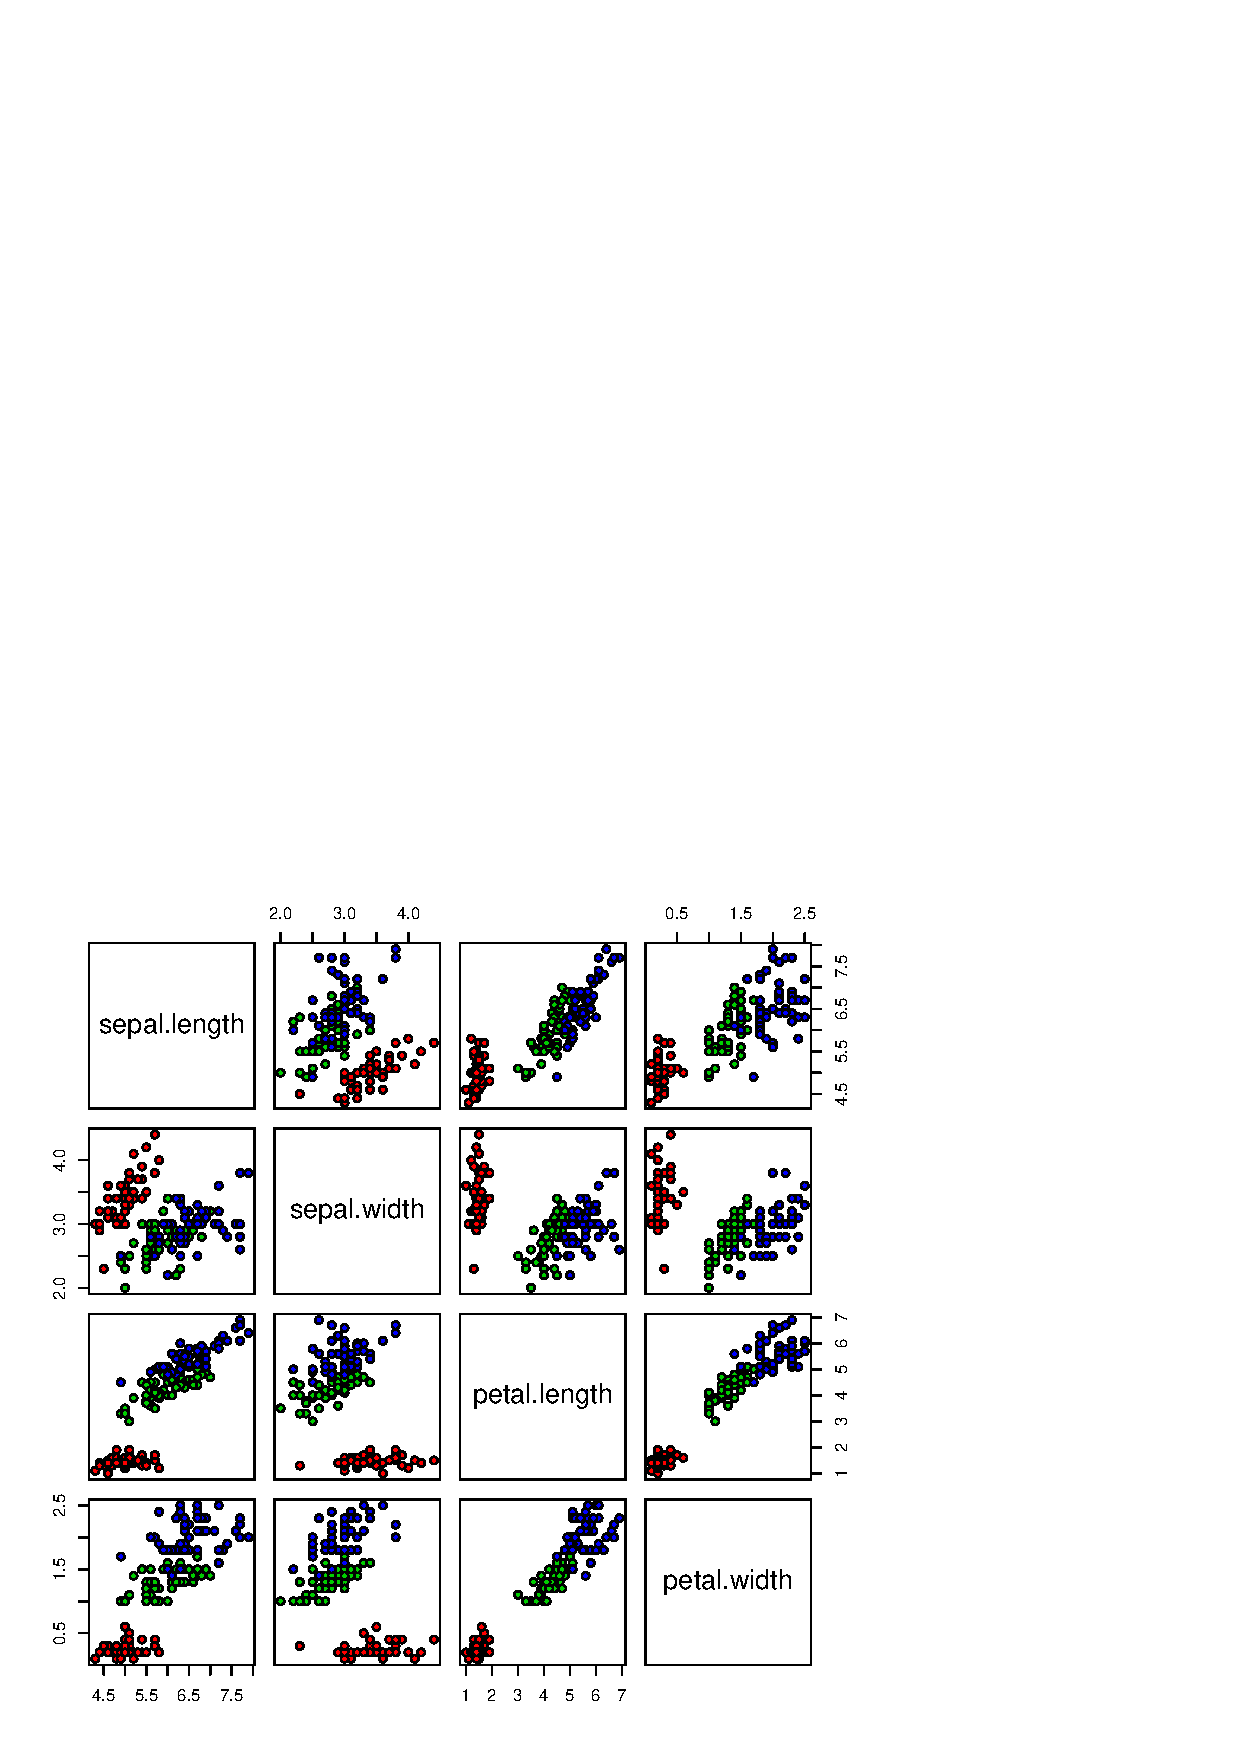
\includegraphics[width=0.8\textwidth]{images/ml/iris-flower-dataset}
  \end{center}
  \caption{Визуализация набора данных ``Ирисы Фишера''. setosa — красный, versicolor — зелёный, virginica — синий.}
  \label{ml:fig:iris-dataset-visualization}
\end{figure}
}

На \autoref{ml:fig:iris-dataset-kmeans} иллюстрирован возможный результат алгоритма $k$ средних.

\IfNotDraft
{
\begin{figure}[tb]
  \begin{center}
    \leavevmode
    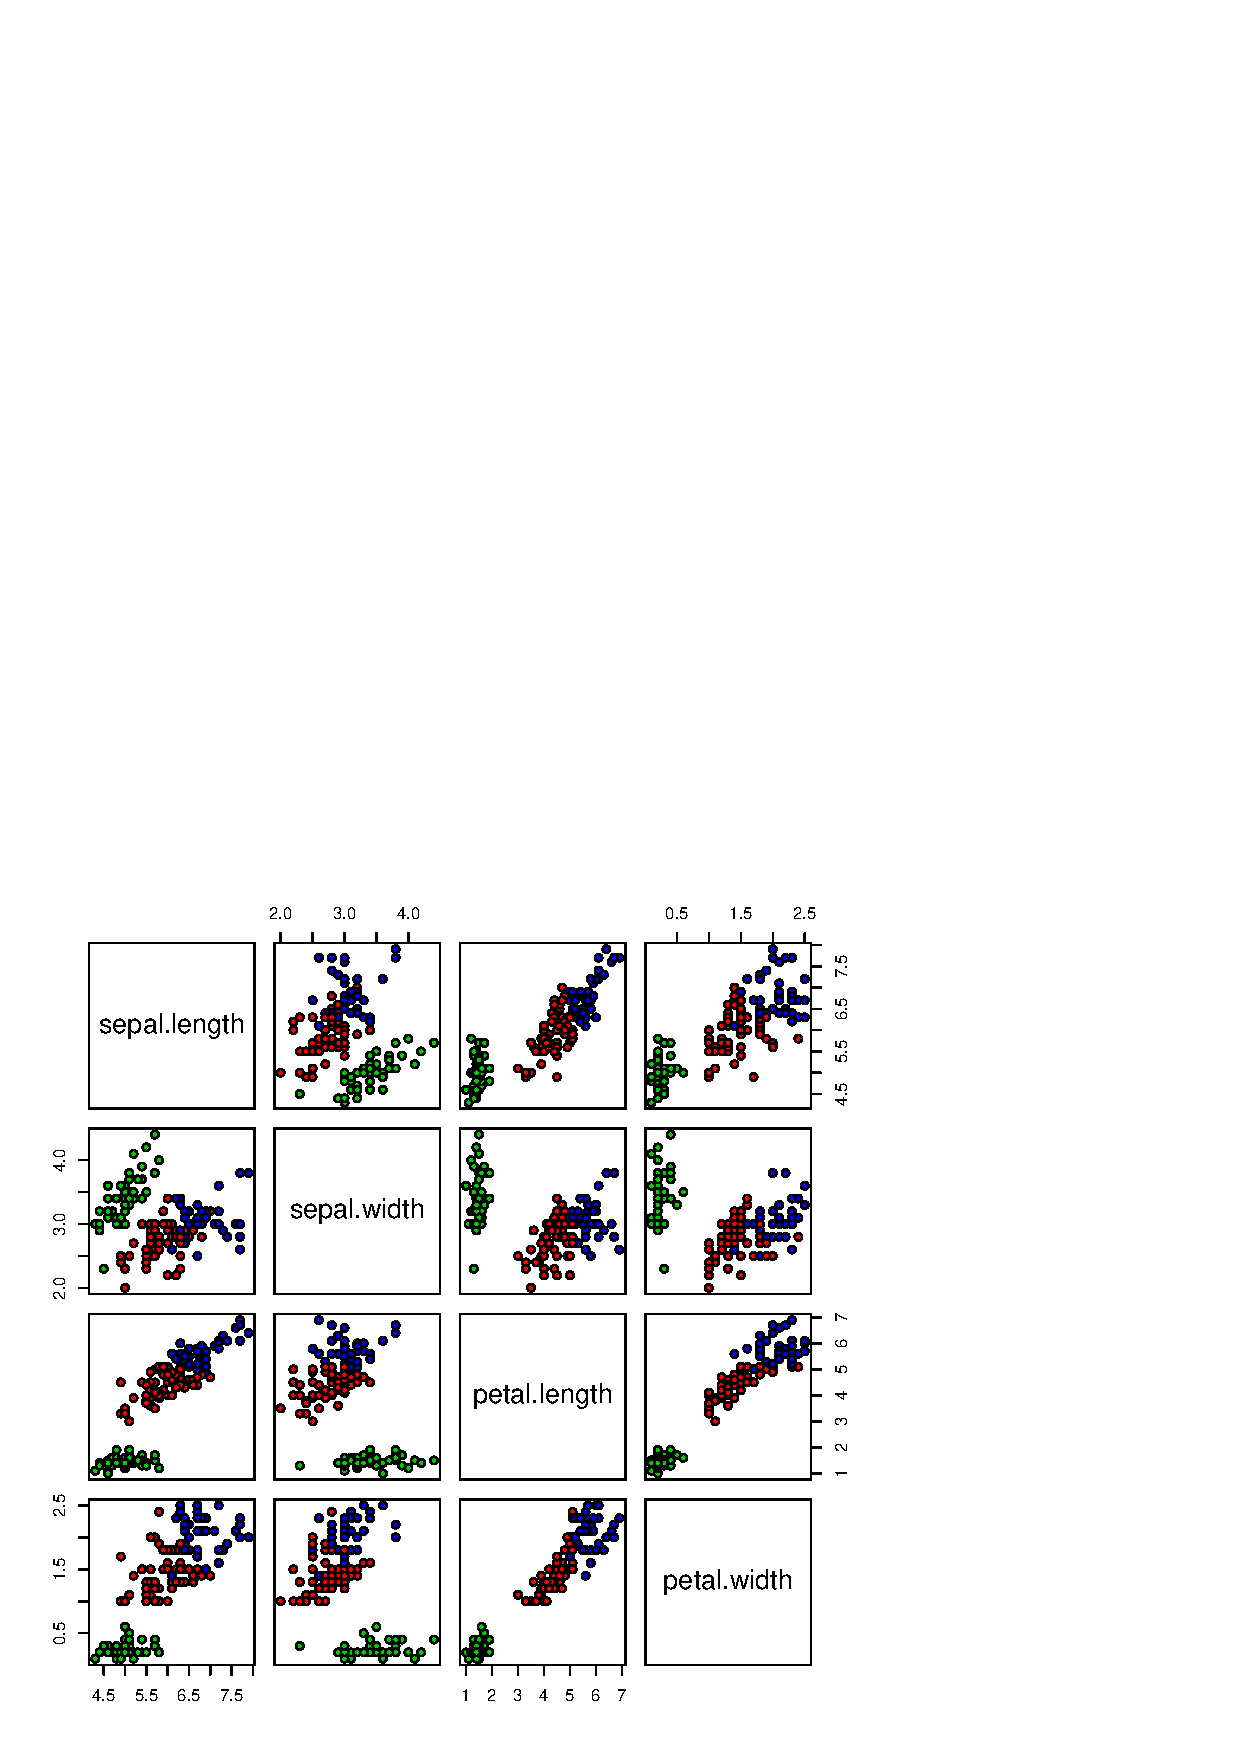
\includegraphics[width=0.8\textwidth]{images/ml/iris-flower-kmeans}
  \end{center}
  \caption{Визуализация клустеризации набора данных ``Ирисы Фишера''.}
  \label{ml:fig:iris-dataset-kmeans}
\end{figure}
}

\section{Классификация}
\emph{Классификация} объекта — это указание класса для данного объекта. Например, по значениям длин и ширин чашелистника и лепестка цветка ириса нужно определить его вид.

\subsection{Метод $k$ ближайших соседей}
Суть \emph{метода $k$ ближайших соседей} (англ. k-nearest neighbor algorithm) состоит в том, что объекту присваивается тот класс, который является наиболее распространённым среди его $k$ соседей. Из этого следует, что нужно иметь набор данных с заранее известными классами объектов.

Для определения близости, как правило, используется евклидова метрика.

Предельно наивная реализация данного алгоритма — предельно очевидна. Она же — приведена ниже:
\begin{pylst}{Наивная реализация kNN}{}
def knn(item, dataset):
    klass = None
    nearest = None

    for row in dataset:
        next = metrics.sim_distance(item, row["features"])

        if nearest is None:
            nearest =  next
        elif next > nearest:
            klass = row["class"]
            nearest = next

    return klass
\end{pylst}

Пример запуска для набора данных ``Ирисы Фишера'':
\begin{pylst}{}{}
>>> knn([4.5, 3.8, 1.2, 0.4], dataset)
"setosa"
\end{pylst}

\subsection{kd деревья}
\emph{kd дерево} (англ. k-dimensional tree) — структура данных, используемая для разбития $k$-размерного пространства на подпространства по некоторым заданных точкам.

kd дерево — это бинарное дерево, в котором каждый узел содержит точку пространства размерности $k$. Каждый внутренний узел представляет собой точку, через которую проходит гиперплоскость, разбивающая пространство на две части. При этом точки из левого поддерева находятся по одну сторону от этой гиперплоскости, точки же правого поддерева — по другую.

Направление гиперплоскостей выбирается следующим образом: выбирается какая-либо ось, и гиперплоскость строится перпендикулярно к этой оси. Например, допустим выбрана ось $x$, тогда все точки текущего поддерева, у которых координата по оси $x$ меньше, будут находится по одну сторону от гиперплоскости, проведённой через точку $(x_{concrete}, 0, \dots)$; оставшиеся же точки — по другую сторону. При этом первые — будут в левом поддереве, вторые же — в правом.

\subsubsection{Построение kd дерева}
Так как способов выбирать следующую ось, перпендикулярно которой строится следующая гиперплоскость, — много, то и построений может быть — много. Каноническим способом является:
\begin{itemize}
  \item Циклически и последовательно выбирать следующую ось по порядку, начиная с оси $x$, для каждого следующего уровня дерева.
  \item Элементом текущего узла является точка, которая является медианой точек текущего поддерева.
\end{itemize}

Посмотрим дерево для точек $(2; 3), (5; 4), (9; 6), (4; 7), (8; 1), (7; 2)$. Оно будет выглядеть, как на \autoref{ml:knn:kdtree-pic}. На плоскости же его можно изобразить, как на \autoref{ml:knn:kdtree-2d}.

\begin{figure}[htb]
  \centering
  \begin{tikzpicture}[xNode/.style={circle,draw,red},
                      yNode/.style={circle,draw,blue},
                      justNode/.style={circle,draw,black},
                      level distance=1.5cm,
                      level/.style={sibling distance=2.5cm/#1},
                      font=\footnotesize]
    \node [xNode] at (0,0) {$7; 2$}
      child { node [yNode] {$5; 4$}
        child { node [justNode] {$2; 3$} }
        child { node [justNode] {$4; 7$} } }
      child { node [yNode] {$9; 6$}
        child { node [justNode] {$8; 1$} } };
  \end{tikzpicture}
  \caption{Пример kd дерева.}
  \label{ml:knn:kdtree-pic}
\end{figure}

\begin{figure}[htb]
  \centering
  \begin{tikzpicture}
    \begin{axis}[
      xlabel=$x$,
      ylabel=$y$,
      xmin=0, xmax=10,
      ymin=0, ymax=10]

      \draw [red] (axis cs:7,0)
        -- (axis cs:7,10);

      \draw [blue] (axis cs:0,4)
        -- (axis cs:7,4);

      \draw [blue] (axis cs:7,6)
        -- (axis cs:10,6);

      \addplot[
        scatter/classes={
          x={mark=square*,red},%
          y={mark=square*,blue},%
          n={mark=square*,black}
        },
        scatter,only marks,
        scatter src=explicit symbolic]
        coordinates {
          (7,2) [x]
          (5,4) [y]
          (9,6) [y]
          (2,3) [n]
          (4,7) [n]
          (8,1) [n]
        };
    \end{axis}
  \end{tikzpicture}
  \caption{Изображение kd дерева на плоскости.}
  \label{ml:knn:kdtree-2d}
\end{figure}

Ниже приведена реализация построения kd дерева из массива вышеупомянутых точек.

\begin{pylst}{}{}
class Node(object):
    def __init__(self, location, kind, left, right):
        self.location = location
        self.kind = kind
        self.left = left
        self.right = right

def kdtree(dataset, depth=0):
    if not dataset:
        return None

    n = len(dataset)
    k = len(dataset[0]["features"])
    axis = depth % k
    median = n // 2

    dataset.sort(key=lambda row: row["features"][axis])

    location = dataset[median]["features"]
    kind = dataset[median]["class"]
    left = kdtree(dataset[:median], depth + 1)
    right = kdtree(dataset[median + 1:], depth + 1)

    return Node(location, kind, left, right)
\end{pylst}

Асимптотическая сложность операций следующая:
\begin{itemize}
  \item Построение из $n$ точек — $O(n \log^2 n)$.
  \item Вставка точки — $O(\log n)$.
  \item Удаление точки — $O(\log n)$.
  \item Поиск ближайшей точки — $O(\log n)$ — в среднем; $O(k \cdot n^{1 - \frac{1}{k}})$ — в худшем случае.
\end{itemize}


\end{document}
